%%
%% Copyright 2007, 2008, 2009 Elsevier Ltd
%%
%% This file is part of the 'Elsarticle Bundle'.
%% ---------------------------------------------
%%
%% It may be distributed under the conditions of the LaTeX Project Public
%% License, either version 1.2 of this license or (at your option) any
%% later version.  The latest version of this license is in
%%    http://www.latex-project.org/lppl.txt
%% and version 1.2 or later is part of all distributions of LaTeX
%% version 1999/12/01 or later.
%%
%% The list of all files belonging to the 'Elsarticle Bundle' is
%% given in the file `manifest.txt'.
%%

%% Template article for Elsevier's document class `elsarticle'
%% with numbered style bibliographic references
%% SP 2008/03/01
%%
%%
%%
%% $Id: elsarticle-template-num.tex 4 2009-10-24 08:22:58Z rishi $
%%
%%
\documentclass[preprint,12pt]{elsarticle}

%% Use the option review to obtain double line spacing
%% \documentclass[preprint,review,12pt]{elsarticle}

%% Use the options 1p,twocolumn; 3p; 3p,twocolumn; 5p; or 5p,twocolumn
%% for a journal layout:
%% \documentclass[final,1p,times]{elsarticle}
%% \documentclass[final,1p,times,twocolumn]{elsarticle}
%% \documentclass[final,3p,times]{elsarticle}
%% \documentclass[final,3p,times,twocolumn]{elsarticle}
%% \documentclass[final,5p,times]{elsarticle}
%% \documentclass[final,5p,times,twocolumn]{elsarticle}

%% if you use PostScript figures in your article
%% use the graphics package for simple commands
%% \usepackage{graphics}
%% or use the graphicx package for more complicated commands
%% \usepackage{graphicx}
%% or use the epsfig package if you prefer to use the old commands
%% \usepackage{epsfig}

%% The amssymb package provides various useful mathematical symbols
\usepackage{amssymb}
%% The amsthm package provides extended theorem environments
%% \usepackage{amsthm}

%% The lineno packages adds line numbers. Start line numbering with
%% \begin{linenumbers}, end it with \end{linenumbers}. Or switch it on
%% for the whole article with \linenumbers after \end{frontmatter}.
%% \usepackage{lineno}

%% natbib.sty is loaded by default. However, natbib options can be
%% provided with \biboptions{...} command. Following options are
%% valid:

%%   round  -  round parentheses are used (default)
%%   square -  square brackets are used   [option]
%%   curly  -  curly braces are used      {option}
%%   angle  -  angle brackets are used    <option>
%%   semicolon  -  multiple citations separated by semi-colon
%%   colon  - same as semicolon, an earlier confusion
%%   comma  -  separated by comma
%%   numbers-  selects numerical citations
%%   super  -  numerical citations as superscripts
%%   sort   -  sorts multiple citations according to order in ref. list
%%   sort&compress   -  like sort, but also compresses numerical citations
%%   compress - compresses without sorting
%%
%% \biboptions{comma,round}

% \biboptions{}


\journal{NIMA}

\begin{document}

\begin{frontmatter}

%% Title, authors and addresses

%% use the tnoteref command within \title for footnotes;
%% use the tnotetext command for the associated footnote;
%% use the fnref command within \author or \address for footnotes;
%% use the fntext command for the associated footnote;
%% use the corref command within \author for corresponding author footnotes;
%% use the cortext command for the associated footnote;
%% use the ead command for the email address,
%% and the form \ead[url] for the home page:
%%
%% \title{Title\tnoteref{label1}}
%% \tnotetext[label1]{}
%% \author{Name\corref{cor1}\fnref{label2}}
%% \ead{email address}
%% \ead[url]{home page}
%% \fntext[label2]{}
%% \cortext[cor1]{}
%% \address{Address\fnref{label3}}
%% \fntext[label3]{}

\title{Particle ID performance of Liquid Argon TPC}

%% use optional labels to link authors explicitly to addresses:
%% \author[label1,label2]{<author name>}
%% \address[label1]{<address>}
%% \address[label2]{<address>}

\author{J-PARC T32 collaboration}

\address{}

\begin{abstract}
%% Text of abstract

This paper describes a study of particle identification performance of
liquid Argon TPC (LArTPC) detector using well-defined charged particles
(pions, kaons, and protons) with momentum of ~800 MeV/$c$
obtained at J-PARC K1.1Br beamline.

We have build a LArTPC detector with fiducial mass of ~150 kg,
and injected the beam particle

\end{abstract}

\begin{keyword}
%% keywords here, in the form: keyword \sep keyword

%% MSC codes here, in the form: \MSC code \sep code
%% or \MSC[2008] code \sep code (2000 is the default)

\end{keyword}

\end{frontmatter}

%%
%% Start line numbering here if you want
%%
% \linenumbers

%% main text
%%%%%%%%%%%%%%%%%%%%%%%%%%%%%%%%%%%%%%%%%%%%%%%%%%
%\section{Introduction}
%%%%%%%%%%%%%%%%%%%%%%%%%%%%%%%%%%%%%%%%%%%%%%%%%%
%%%%%%%%%%%%%%%%%%%%%%%%%%%%%%%%%%%%%%%%%%%%%%%%%%
\section{Introduction}
%%%%%%%%%%%%%%%%%%%%%%%%%%%%%%%%%%%%%%%%%%%%%%%%%%
Refer \cite{Araoka:2011pw} for hardware/beam line description

%%%%%%%%%%%%%%%%%%%%%%%%%%%%%%%%%%%%%%%%%%%%%%%%%%
%\section{Data Quality}
%%%%%%%%%%%%%%%%%%%%%%%%%%%%%%%%%%%%%%%%%%%%%%%%%%

%%%%%%%%%%%%%%%%%%%%%%%%%%%%%%%%%%%%%%%%%%%%%%%%%%
\section{Data Quality}
%%%%%%%%%%%%%%%%%%%%%%%%%%%%%%%%%%%%%%%%%%%%%%%%%%
\subsection{Collected Data}

Table~\ref{Table:Data} shows list of the collected data while Oct/2010 Run.
800 MeV/$c$ pion is expected to pass-through the detector as MIP,
and have uniform energy deposition to all the TPC channels.
So this data set is very useful for calibrating the detector response (See section xxx).
800 MeV/$c$ proton stops after ~15 cm of flight distance inside the TPC fiducial volume
with relatively large $dE/dx$. So we use the proton data set for validation of the
detector response at high $dE/dx$ region(See section xxx).
We have collected three different Kaon data by varying thickness of the degrader. 
540, 630, 680 MeV/$c$ are corresponds to the momentum degraded by 
2 lead glass, 1 lead glass + 1 lead block, and 1 lead glass, respectively, 
and such Kaon stops after 10 cm, 50 cm, and 65 cm of flight distance inside TPC fiducial volume.

Figure~\ref{Fig:Textbook} shows an 2D display of typical event 
taken with 800 MeV/$c$ electron trigger.
Horizontal axis corresponds to TPC channel number 
and zero means most upper stream strip. 
Since strip pitch is 1 cm, this is equivalent to
distance from beam injection point in cm.
Vertical axis corresponds to electron drift time in $\mu$s
and t=0 means trigger timing. In this TPC, anode and cathode is
located at top and bottom of the detector, respectively,
t=0 means energy deposition at anode and longer drift time 
means energy deposition in lower height.
With 200 V/cm of electric field, drift velocity is about 0.8 m/ms.
So drift of full detector (40 cm) takes 500 $\mu$s.
Color strength of the plot corresponds to the TPC signal pulse height
in ADC counts which is roughly proportional to $dE/dx$ of the track.
In this event, triggered electron can be clearly seen center of the detector
as an electromagnetic shower while there are two other particles 
accidentally overlapped with the triggered electron. 
Track at t=100 $\mu$s is considered as
a proton which stops after 15 cm of flight distance and 
has large $dE/dx$ around the stopped point.
Track at t=400 $\mu$s is considered as
a pion which passes-through the detector and 
has uniform $dE/dx$ over the TPC channels.
This event already gives us some idea for how good 
the particle identification performance of the LArTPC is.

Figure~\ref{Fig:Kmunu} shows a typical $K \to\mu\nu$ like event.
We can clearly identify a kink of the track at 60 cm which is considered
as stopped point of Kaon and it decays to  

Energy deposition of the track is about MIP at the injection point
and gradually increase towards the stopped point at 60 cm.



\begin{table}[h]
\begin{center}
\caption{List of collected data}
\begin{tabular}{l|ll}
  Particle  &Momentum (MeV/$c$) &Number of Events\\
\hline
  Pion      &800                &3,000\\
  Proton    &800                &1,500\\
  Kaon      &540 (2LG)          &7,000\\
  Kaon      &630 (1LG+1LB)      &40,000\\
  Kaon      &680 (1LB)          &35,000\\
  electron  &800                &2,500\\
  electron  &200                &10,000\\
  pion      &200                &10,000\\
\end{tabular}
\label{Table:Data}
\end{center}
\end{table}



\begin{figure}[htbp]
 \begin{center}
  \includegraphics[width=100mm]{fig/Textbook.eps}
 \end{center}
 \caption{Event display of 800 MeV/$c$ electron triggered event.
Accidentally overlapped with a proton and a pion.}
 \label{Fig:Textbook}
\end{figure}

\begin{figure}[htbp]
 \begin{center}
  \includegraphics[width=100mm]{fig/Kmunu.eps}
 \end{center}
 \caption{Event display of Kaon 630 MeV/$c$ triggered event}
 \label{Fig:Kmunu}
\end{figure}

\subsection{Beam Quality (Purity)}
\begin{itemize}
\item Plot: TREK counters (FC, GC, TOF) (A. Okamoto)
\item Plot: TOF before and after selection  (A. Okamoto)
\end{itemize}

 As described in section xx, we have several beam counters
to identify beam particles event by event
Figure~ref{fig:TREK} shows response of the, FC, GC, and TOF counters.
By using these counter information,

\begin{table}[h]
\begin{tabular}{llll}
  Particle  &FC(K) &FC(pi) &GC\\
  Pion      &x     &o      &x\\
  Kaon      &o     &x      &x\\
  Proton    &o     &x      &x\\
  electron  &x     &o      &o\\

\end{tabular}
\caption{List of collected data}
\label{Table:Data}
\end{table}


GC is used to identify electrons
 
\subsection{Beam Energy, Position}
   \subsection{Beam Energy}
 
   30GeV proton beam hits to target T1 in Hadron hall.
   It generates many particles like kaon, pion, muon, electron, and
   so on.
   We take the particles that has 800MeV/c momentum from this beam by
   using D1 magnet.\\
   \ \ For this analysis, a beam momentum at BDC after passing through the
   K1.1Br beam line is required.
   We estimate a beam momentum using simple MC simulation.
   Figure \ref{K11Br_Beam_line} shows MC simulation's geometory.
   This time, beam line is straight and has no electric and magnetic
   field.
   MC simulation shoot 800MeV/c kaon and pion as pencil beam.

   Figure \ref{k_pi_momentum} shows kaon and pion momentum distribution
   using this MC simulation.
   Actually, kaon momentum distribution peak is adjusted so that kaon
   decay point of MC simulation is consistent with data.
   Section \ref{kaon_energy_section} explains this point.
   And proton momentum is estimated in other way, using TREK detector
   TOF information.
   Section \ref{proton_energy_section} shows proton momentum distribution.

   \subsubsection{Kaon energy}\label{kaon_energy_section}

We adjust momentum peak of figure ?? and set Kaon beam energy  the point that the decay points of Kaon in data and simulation are good agreement. The distribution of decay poins are plotted in Figure\ref{DecayPoint_hough}.
\begin{figure}[!htb]
  \begin{center}
    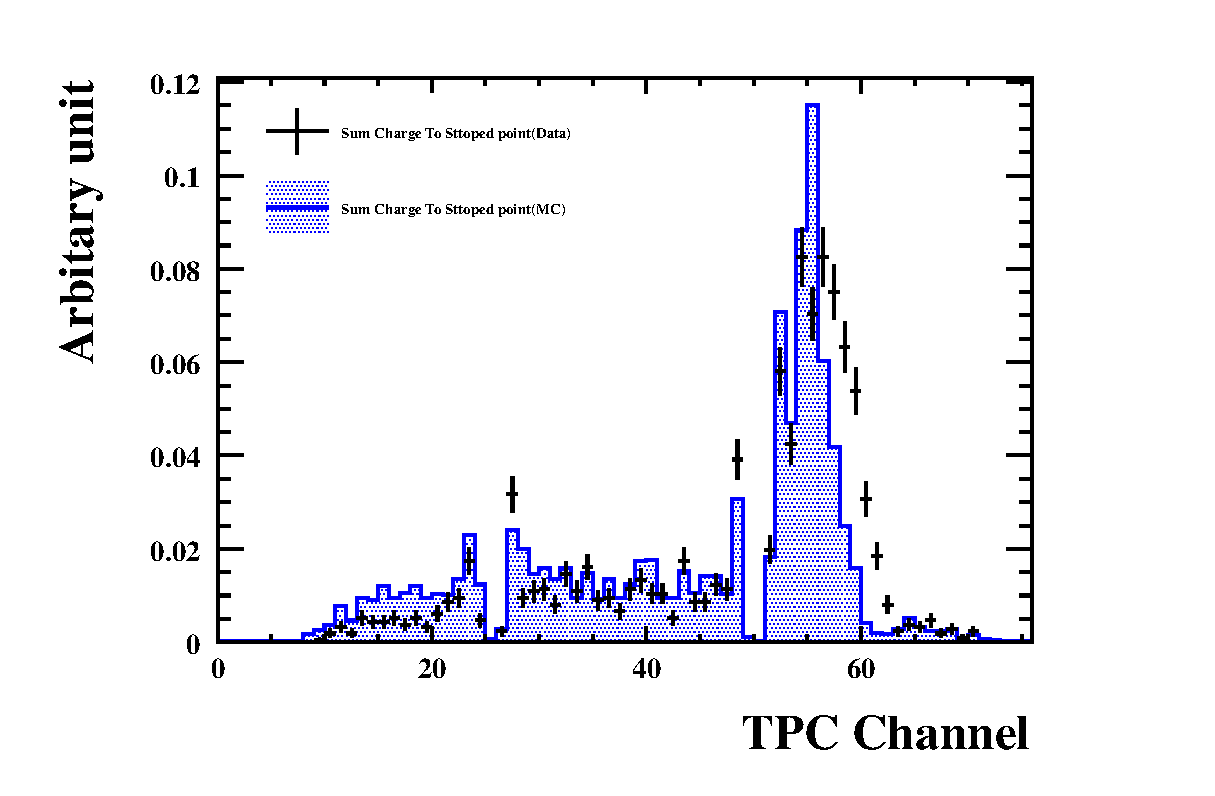
\includegraphics[width=70mm]{fig/cdp_hough.eps}
  \end{center}
  \caption{Decay point distribution of Data and MC}
  \label{DecayPoint_hough}
\end{figure}

   \subsubsection{Proton energy}\label{proton_energy_section}

Beam momentum is ideally TOF information,
but considered the dispersion, we should take into account of the resolution of TOF.
As we know the resolution of TOF is $\sim$200ps beforehand,
we can calculate the effect of this resolution to beam momentum.
For example, as shows in table\ref{tb:TOF_expect}, 
the time of flight of 800MeV/c $K^{+}$ between two TOF Counters is 13.71$ns$.
When considering 0.2$ns$ TOF resolution for this value,
the momentum is approximately 760$\sim$845MeV/c spreading largely.
However, taking the same calculation for 800MeV/c $p$,
the momentum is approximately 785$\sim$815MeV/c surpressing the dispersion to some extent.
In addition, because the dispersion of Time of Flight of $p$ appears widespread over TOF resolution,
we estimate the momentum of $p$ from TOF information.\\
Figure\ref{fig:Proton_tof} shows responce of TOF Counters of PhysicsOct49 whose data include many $p$ events.
As discribed above, the holizontal axis don't show the real time of flight.
Then, with PhysicsOct47 whose data include much $e^{+}$ events, we determined the mean of $e^{+}$.
As the $beta$ of $e^{+}$ is $\sim$1.0, this value of horizontal axis correspond 11.67$ns$(dotted line in Fig\ref{fig:Proton_tof}).
Figure\ref{fig:Proton_momentum} shows the estimated momentum histgram from figure\ref{fig:Proton_tof}
and this momentum distribution is implemented to Monte Carlo Simulation.
Whether the distribution reproduce DATA well is discussed in section 7.2.

\begin{figure}[htbp]
  \begin{tabular}{cc}
    \begin{minipage}{0.5\hsize}
      \centering
      \includegraphics[width=6cm,clip]{fig/TOF_proton.eps}
      \caption{$p$ TOF response}
      \label{fig:Proton_tof}
    \end{minipage}
    \begin{minipage}{0.5\hsize}
      \centering
      \includegraphics[width=6cm,clip]{fig/Momentum_proton.eps}
      \caption{Estimated $p$ momentum}
      \label{fig:Proton_momentum}
    \end{minipage}
  \end{tabular}
\end{figure} 

   \subsubsection{Energy deposition in degrader}
   Because of having high energy, kaon beam from BDC passes through 250LAr TPC.
   So that kaon stops in 250LAr TPC, we put degrader, which reduce
   beam energy, on beam line.
   In this experiment, we used lead glass and lead block as degrader.
   We estimate energy deposition in degrader by using MC simulation.
   Figure \ref{energy_deposition} shows energy deposition in degrader.
   
   \subsection{Beam Position}
   Before taking data, we measured a beam profile on the front of
   250LAr TPC by using plastic scintillation counter.
   Figure \ref{beamprofile_250L} shows beam profile on the front of
   250LAr TPC.

   \begin{figure}[!htb]
    \centering
    \centering
    \includegraphics[width=11cm,clip]{./fig/K11Br_beamline_sim.eps}
    \caption{K1.1 Br beamline}
    \label{K11Br_Beam_line}
   \end{figure}



   \begin{figure}[!htb]
    \centering
    \centering
    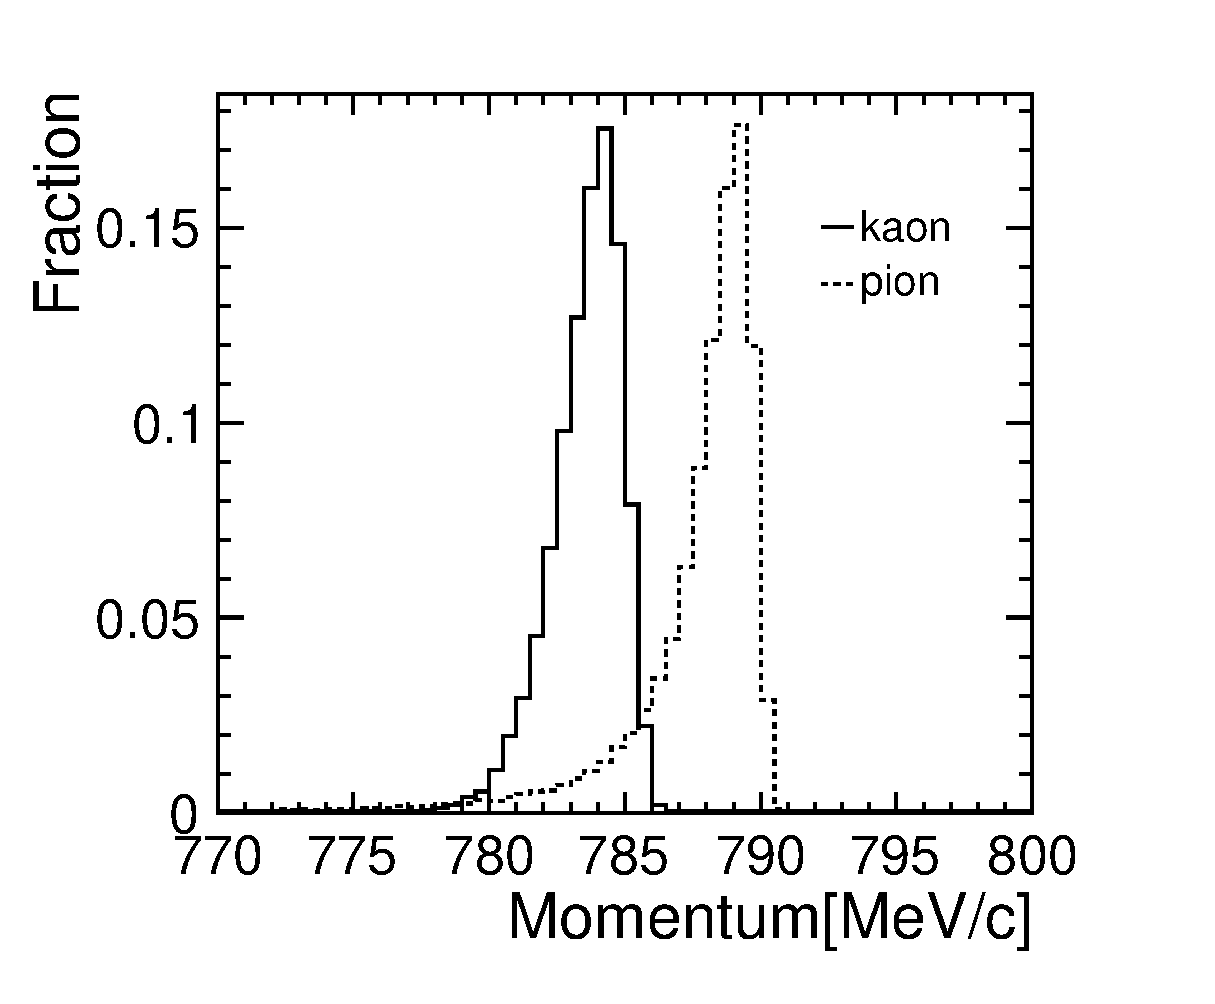
\includegraphics[width=11cm,clip]{./fig/Kaon_pion_momentum_nogrid.eps}
    \caption{kaon and pion momentum distribution at BDC}
    \label{k_pi_momentum}
   \end{figure}


   \begin{figure}[!htb]
    \centering
    \centering
    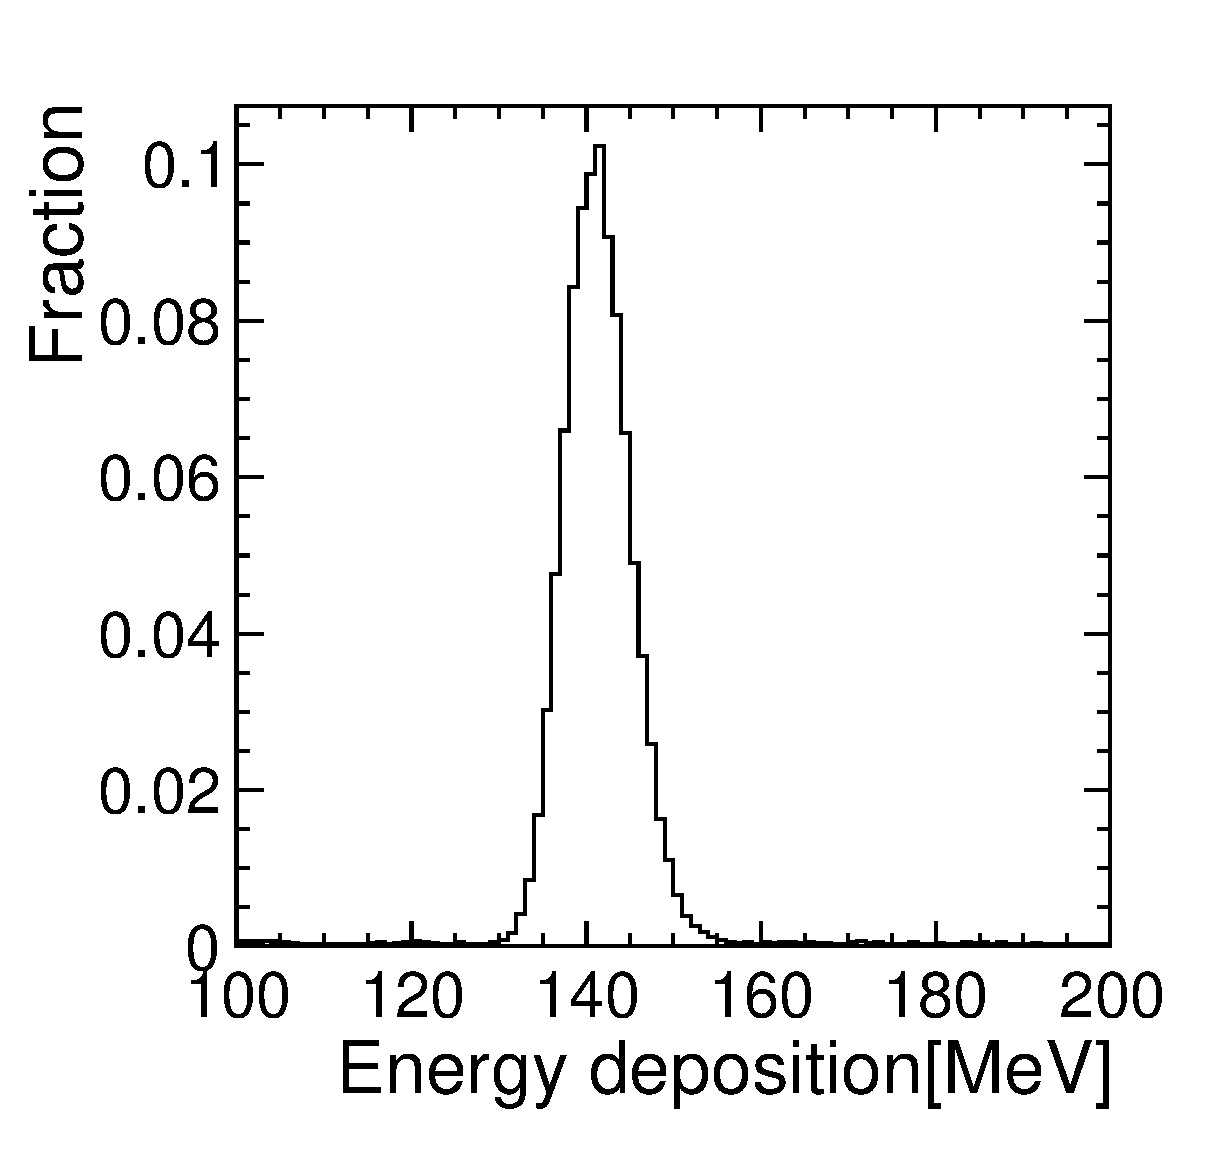
\includegraphics[width=11cm,clip]{./fig/energy_deposition.eps}
    \caption{energy deposition in degrader}
    \label{energy_deposition}
   \end{figure}


   \begin{figure}[!htb]
    \centering
    \centering
    \includegraphics[width=11cm,clip]{./fig/BeamProfile3.eps}
    \caption{Beam profile on the front of 250LAr TPC}
    \label{beamprofile_250L}
   \end{figure}

\begin{itemize}
\item Plot: Proton momentum from TOF  (A. Okamoto)
\item Kaon:: Ongoing  (H. Okamoto?)
\item Plot: Beam position measurement
\end{itemize}


%%%%%%%%%%%%%%%%%%%%%%%%%%%%%%%%%%%%%%%%%%%%%%%%%%
%\section{Software Framework}
%%%%%%%%%%%%%%%%%%%%%%%%%%%%%%%%%%%%%%%%%%%%%%%%%%
%%%%%%%%%%%%%%%%%%%%%%%%%%%%%%%%%%%%%%%%%%%%%%%%%%
\section{Software Framework}
%%%%%%%%%%%%%%%%%%%%%%%%%%%%%%%%%%%%%%%%%%%%%%%%%%
Qscan is a general purpose software package for LArTPC analysis(reference)
which provides,
\begin{itemize}
\item event reconstruction:  noise reduction, hit finding, clustering, and tracking...
\item event simulation: GEANT VMC with ROOT geometry, ionization electron recombination, drift, digitization... 
\item event visualization: display raw data waveform and reconstructed quantities
\end{itemize}

%%%%%%%%%%%%%%%%%%%%%%%%%%%%%%%%%%%%%%%%%%%%%%%%%%
%\section{Event Reconstruction}
%%%%%%%%%%%%%%%%%%%%%%%%%%%%%%%%%%%%%%%%%%%%%%%%%%
%%%%%%%%%%%%%%%%%%%%%%%%%%%%%%%%%%%%%%%%%%%%%%%%%%
\section{Event Reconstruction}
%%%%%%%%%%%%%%%%%%%%%%%%%%%%%%%%%%%%%%%%%%%%%%%%%%
\subsection{Noise Reduction}

Figure \ref{Fig:beforeFFT} shows raw waveform of the TPC signal
before applying any noise reduction. Two waveforms shown in this plot
are channel 13 and 37 in Figure~\ref{Fig:Textbook} which are roughly
proton stopped point and electron shower maximum point, respectively.
Signal-to-noise ratio for this particular case is poor and pion signal 
which is supposed to be t=400 $\mu$s is almost hidden by the noise. 
While time width of TPC signal is few $\mu$s which is determined by
drift time between anode and anode-grid, dominant noise component looks
higher frequency. To reduce such noises, we have applied FFT 
(Fast Flourier Transformation) filter to cut the high frequency component.
Figure \ref{Fig:FFT} shows amplitude as a function of frequency
for the same event. This clearly shows dominant noise component with
$>$ 200 kHz has good separation with signal component ($<$ 100 kHz).
Figure \ref{Fig:afterFFT} shows the waveform after removing high frequency
($>$ 80 kHz) component by the FFT filter. Signal-to-noise ratio is dramatically
improved. On the other hand, we expect certain bias to the signal charge
measurement by this filter, and it will be discussed in Section x.

\begin{figure}[htbp]
 \begin{center}
  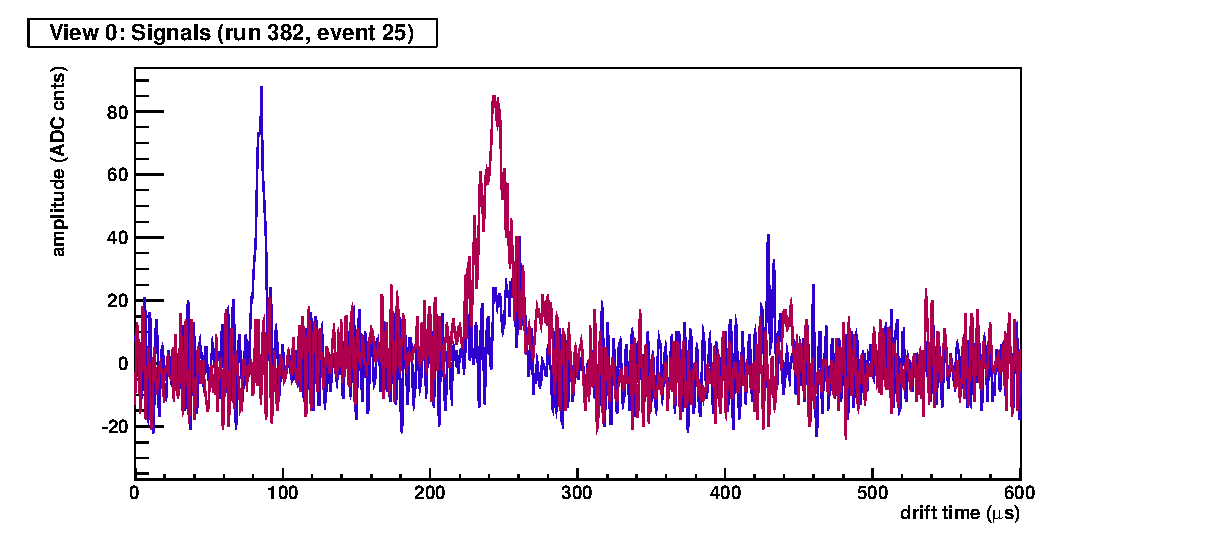
\includegraphics[width=100mm]{fig/beforeFFT.eps}
 \end{center}
 \caption{TPC raw signal waveform for "Textbook" event channel 13 and 37.}
 \label{Fig:beforeFFT}
\end{figure}

\begin{figure}[htbp]
 \begin{center}
  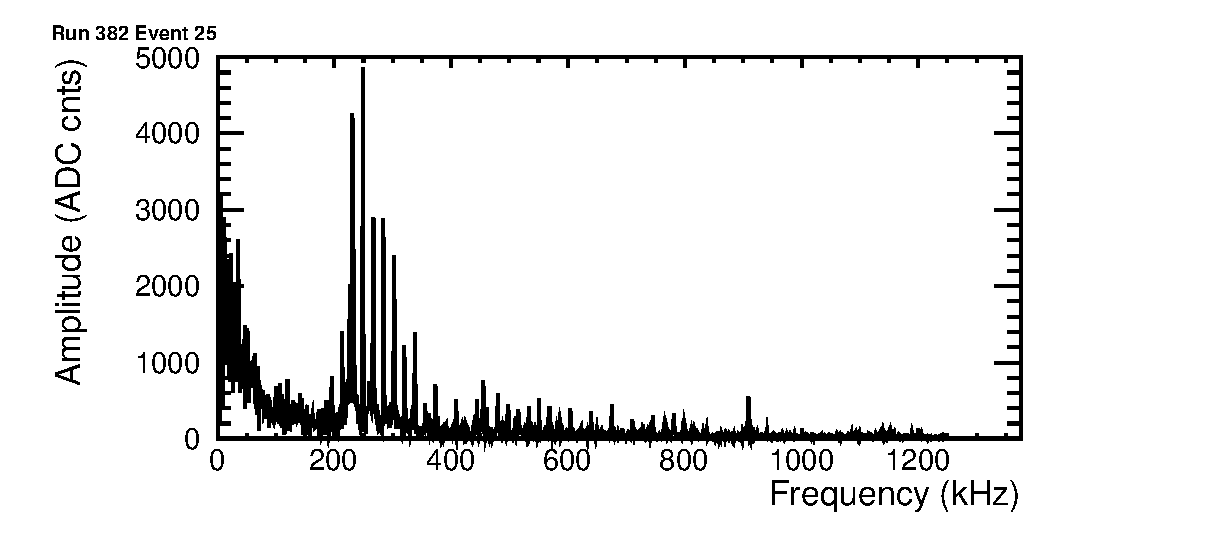
\includegraphics[width=100mm]{fig/FFT.eps}
 \end{center}
 \caption{FFT frequency amplitude distribution}
 \label{Fig:beforeFFT}
\end{figure}

\begin{figure}[htbp]
 \begin{center}
  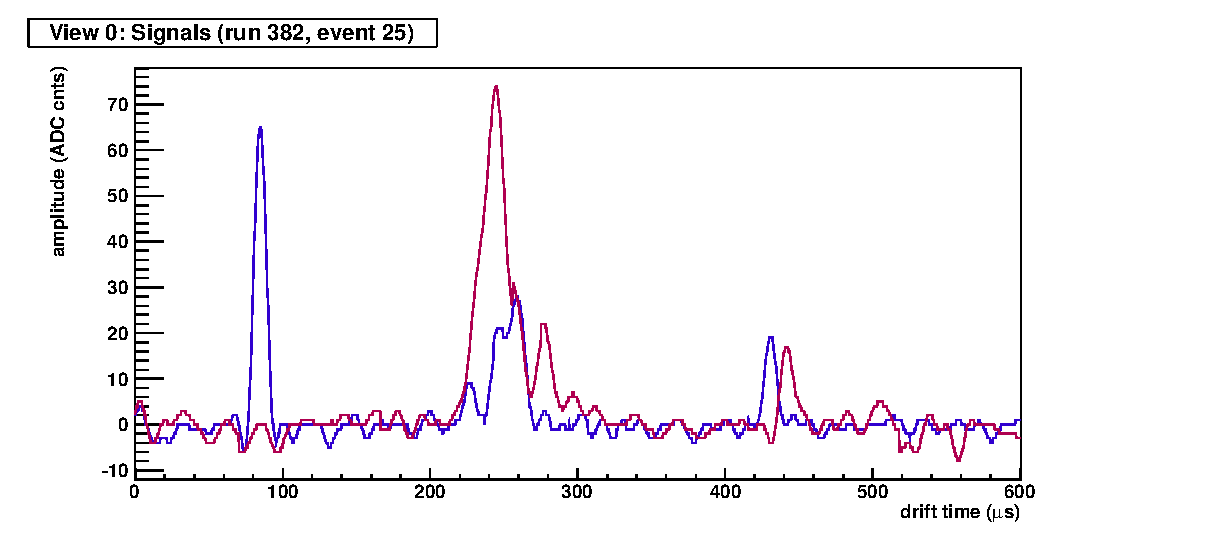
\includegraphics[width=100mm]{fig/afterFFT.eps}
 \end{center}
 \caption{TPC signal waveform after cutting the frequency $>$ 80 kHz.}
 \label{Fig:afterFFT}
\end{figure}


%\subsection{Hit Finding/Clustering}
\subsection{Hit Finding/Clustering}
After noise reduction we find signal hits and create clusters associated to single tracks. 
Hit is defined as bump over given threshold in a channel. 
After finding all hits in an event, we construct cluster by merging adjacent hits. 
The example of hit finding and clustering is shown in Fig~\ref{fig:Clustering}, which indicates reasonable hit and cluster findings. 
Threshold of hit finding is 6 ADC counts, which is about 2.5$\sigma$ from typical data noise level (as shown in Fig~\ref{Fig:beforeFFT}) and keeping more than 99\% of Kaon hit finding efficiency from simulation.
% noise level from outside window of PhysicsOct55 (rms~2.49)
ADC count distribution is fitted by step funcion plus Gaussian to estimate the charge of hit in ADC $\times$ $\mu$s unit.
Fitting $\chi^2 < 3$ and $2.5<$~(time~width~of~hit)~$<8$~$\mu$s are required to remove noise hits further.

\begin{figure}[htbp]
 \begin{center}
  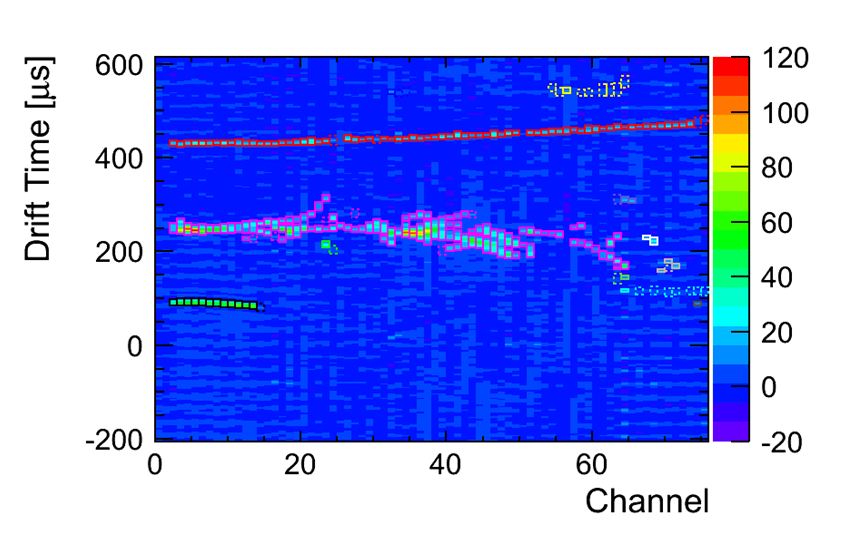
\includegraphics[width=100mm]{fig/clustering.eps}
 \end{center}
 \caption{Example of hit finding and clustering. A colored box corresponds to a hit and colors represent different clusters.}
 \label{fig:Clustering}
\end{figure}

%\begin{itemize}
%\item Plot: Finding efficiency vs threshold (Naganoma): TBU
%\item Plot: Through-going pion data Q vs pion (Tanaka)
%\end{itemize}


\subsection{Stopped Point Finding}
\subsubsection{Proton}
%\subsection{Stopped Kaon}
\subsection{Stopped Kaon}
Hough transform was invented for machine analysis of bubble chamber photographs by Paul.V.C.Hough.\cite{3069654}
We detect straight lines using hough method , and find Kaon stopped point from the intersection of straight lines.\\
Figure \ref{hmap2} shows hit map like a Kaon track.
One point in the X-Y space can be transformed into sinusoidal curve in the $\rho$-$\theta$ space.Figure \ref{rho_theta2} shows sinusoidal curves in all points.
And, we detect the straight line associated with the largest number of points by choosing the most dense point in $\rho$-$\theta$ space.
Next , the sinusoidal curves of the hits associated with frist straight line are removed from figure \ref{rho_theta2}.
Figure \ref{rho_theta3} shows sinusoidal curves after the hits associated with frist straight line removed.
We detect second straight line using the same procedure.This procedure is repeated until there are less than three points.Figure \ref{hmap_fit} shows the two straight lines detected by hough transform mehotd.\\
Kaon stopped point in the liquid argon detecor defined as charge maximum point around the intersection of some lines.


\begin{figure}[!htb]
  \begin{minipage}{0.5\hsize}
    \begin{center}
      \includegraphics[width=35mm]{fig/hmap2.eps}
    \end{center}
    \caption{Hit map like a Kaon track}
    \label{hmap2}
  \end{minipage}
  \begin{minipage}{0.5\hsize}
    \begin{center}
      \includegraphics[width=35mm]{fig/rho_theta2.eps}
    \end{center}
    \caption{sinusoidal curves getting form all hough transformed  points of Figure \ref{hmap2}}
    \label{rho_theta2}
  \end{minipage}
  \\
  \begin{minipage}{0.5\hsize}
    \begin{center}
      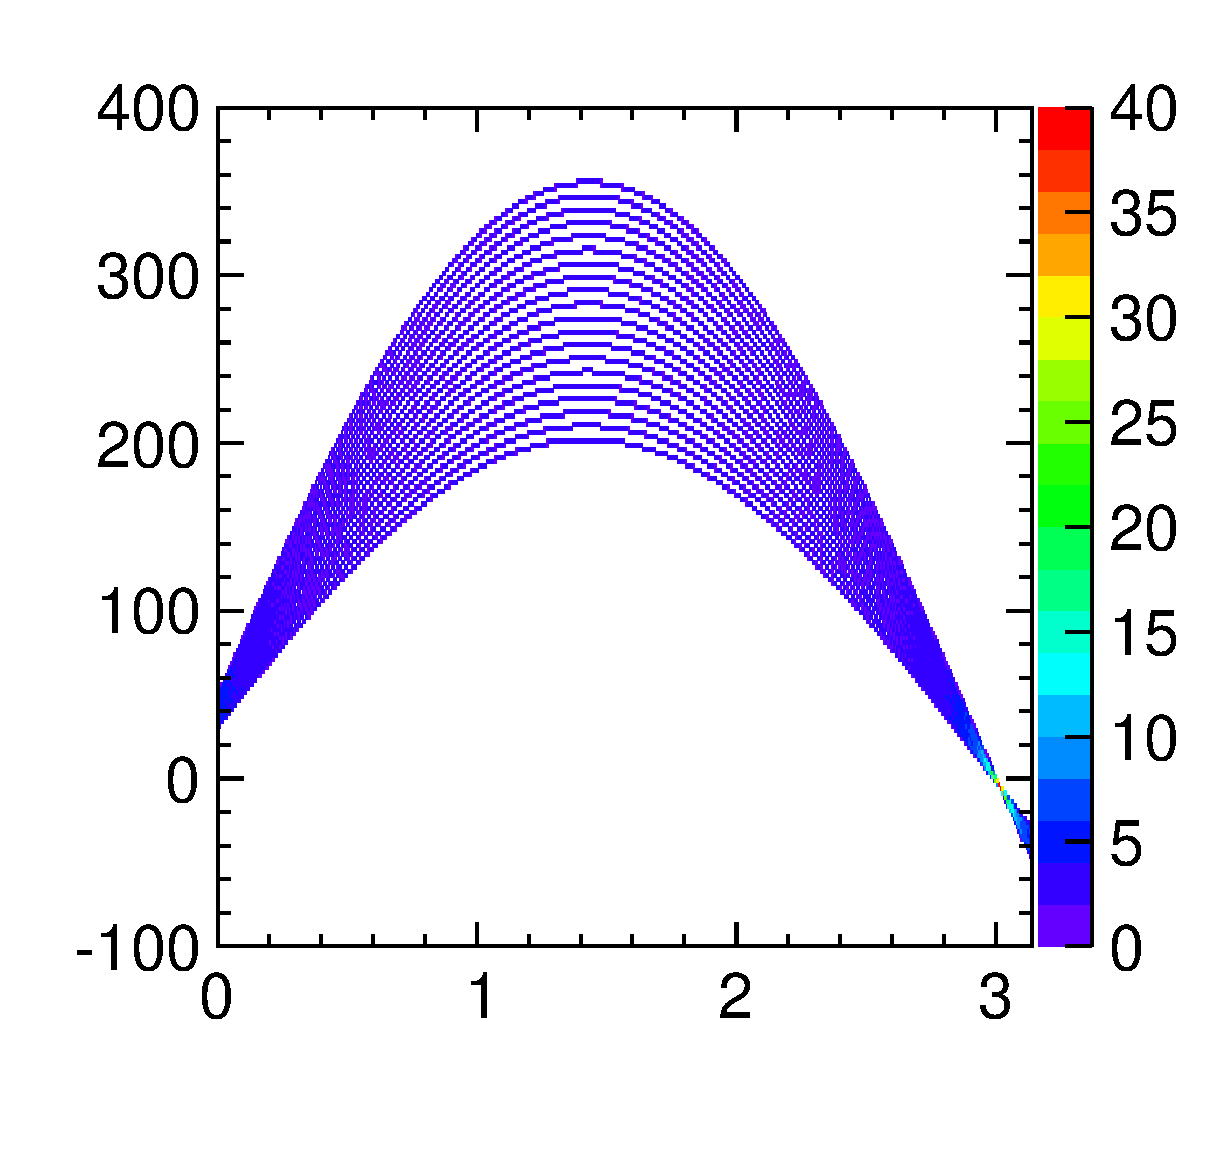
\includegraphics[width=35mm]{fig/rho_theta_kink.eps}
    \end{center}
    \caption{sinusoidal curves removed the points associated with first straight line from figure \ref{rho_theta2}}
    \label{rho_theta3}
  \end{minipage}
  \begin{minipage}{0.5\hsize}
    \begin{center}
      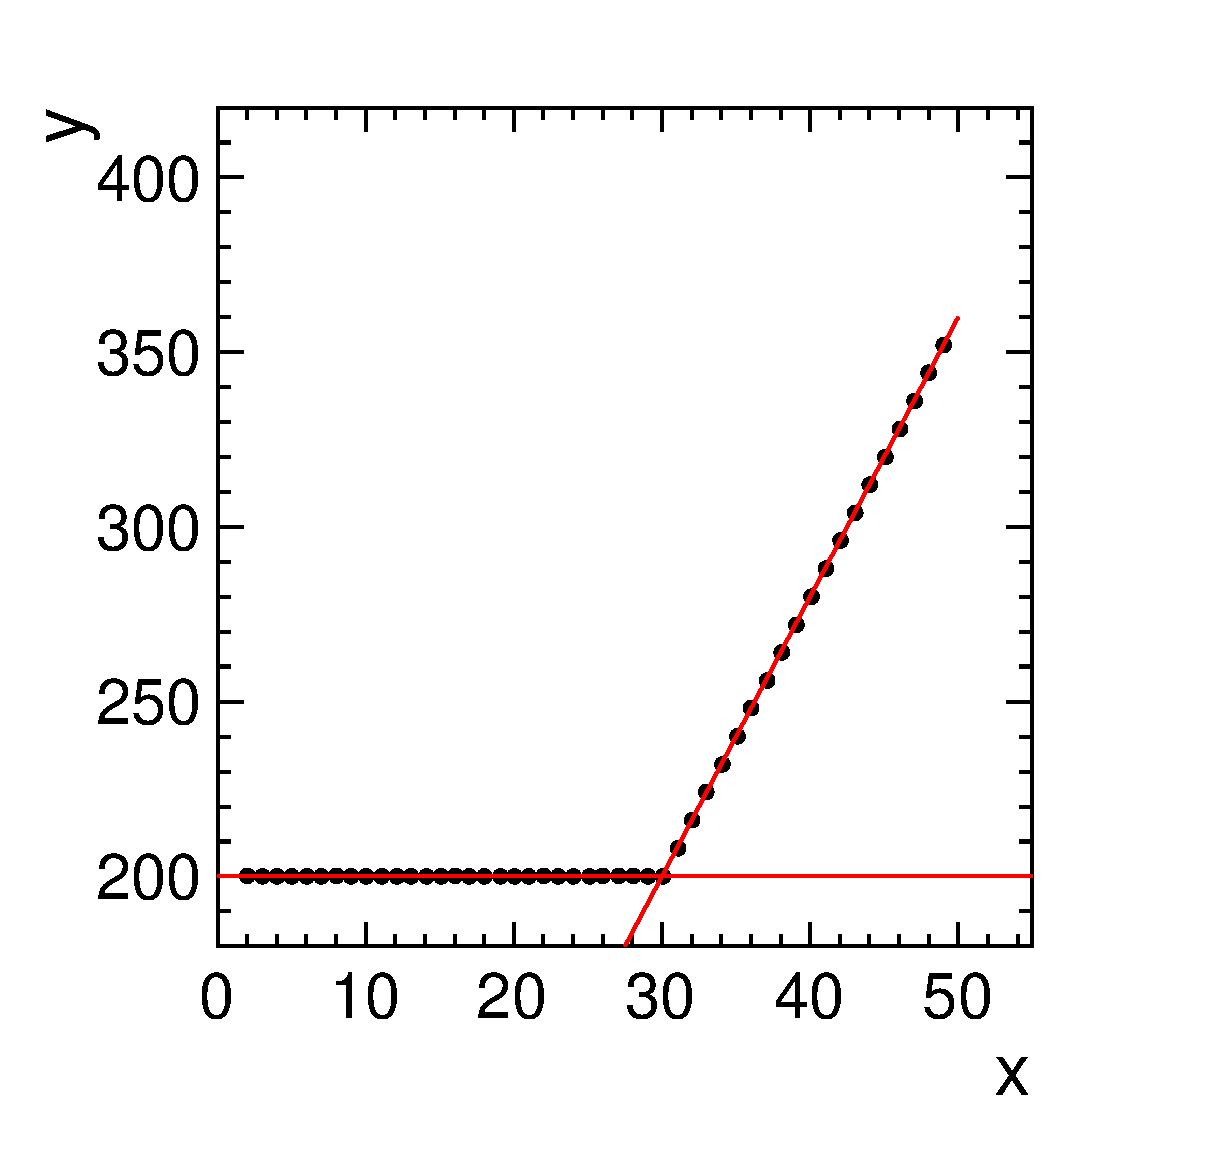
\includegraphics[width=35mm]{fig/hmap_fit.eps}
    \end{center}
    \caption{Two lines detected with hough transform method}
    \label{hmap_fit}
  \end{minipage}
\end{figure}


\subsubsection{Chi2 method}
$\chi^{2}$ method is the algorithm that search the point of rapidly increasing fit'$\chi^{2}$ and the point defined as the stopped point.
Because the charged particle coming from upsteam of beam line , track reconstruction is started from minimum channel  to the maximum channel of the cluster.\\
Figure \ref{hmap3} shows hit map like a Kaon track.
We start fitting with straight line from minimum channel to maximum channel.Figure \ref{xvschi} shows range vs fit'$\chi^{2}$ distribution.
As it can be noiced for figure \ref{xvschi}, $\chi^{2}$ is increased rapidly if the straight line is strayed out.
Then , we search the strayed point from the straight line by setting reasonable threhold and draw from minimum channel to the strayed point.
This procedure is done from maximum channel to minimum channel in the same way.
And we draw from maximum channel to the strayed point.
Kaon stopped point in the liquid argon detecor defined as charge maximum point around the intersection of two lines.


\begin{figure}[!htb]
  \begin{minipage}{0.5\hsize}
    \begin{center}
      \includegraphics[width=50mm]{fig/hmap_kink_chi2.eps}
    \end{center}
    \caption{hit map like a Kaon track}
    \label{hmap3}
  \end{minipage}
  \begin{minipage}{0.5\hsize}
    \begin{center}
      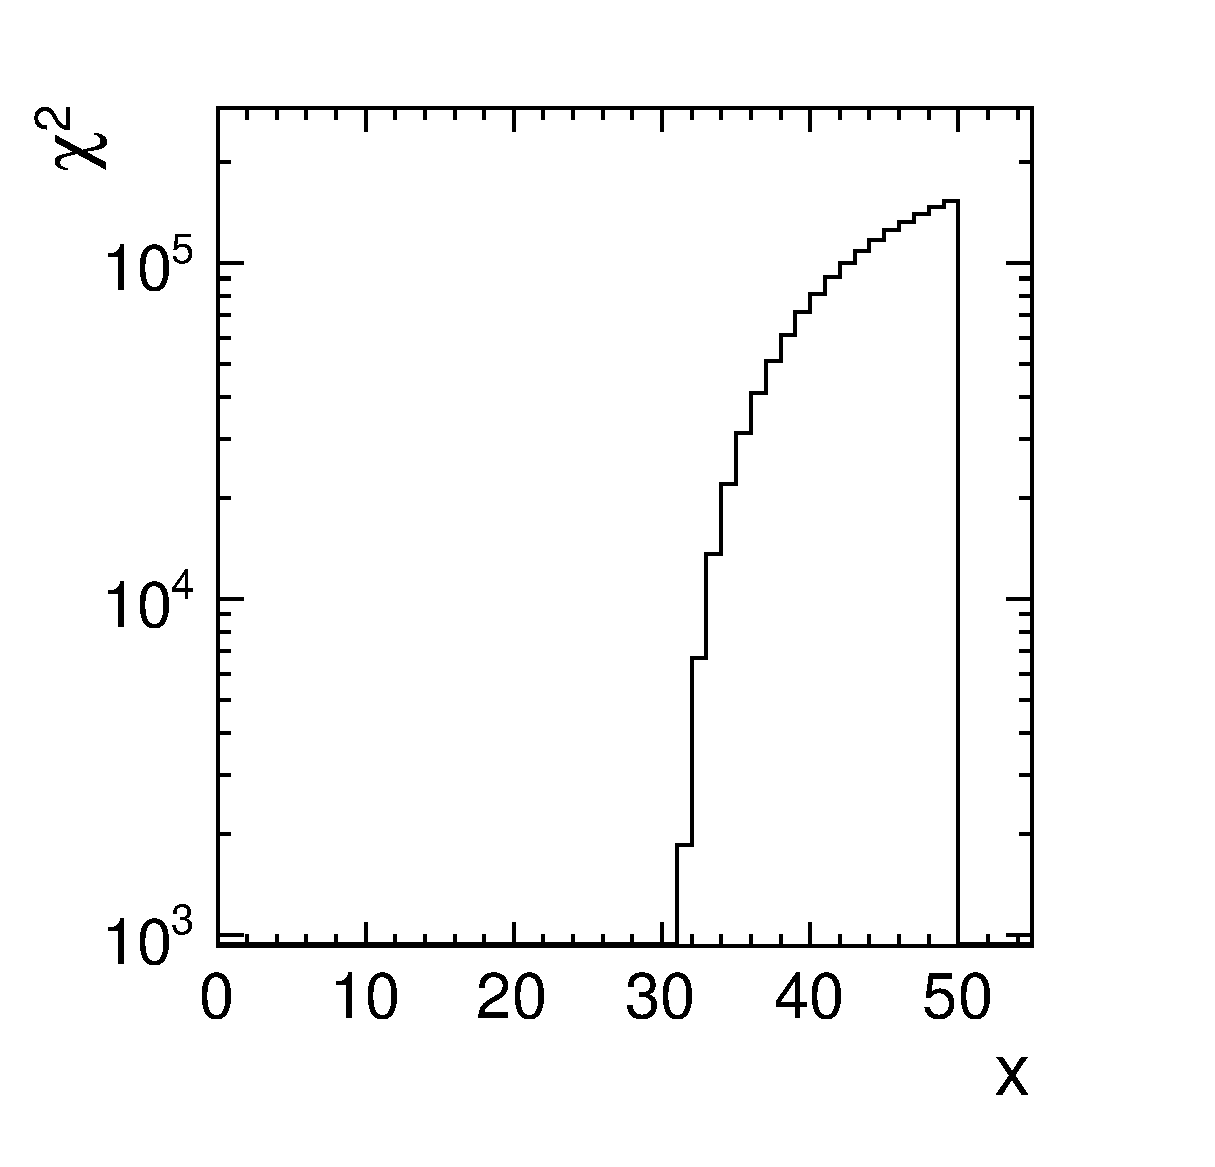
\includegraphics[width=50mm]{fig/chi2_kink_chi2.eps}
    \end{center}
    \caption{range vs $\chi^{2}$ distribution}
    \label{xvschi}
  \end{minipage}
\end{figure}


\subsubsection{BS method}
In the $\chi^{2}$ method , we can't detect Kaon stopped point in the case of backward decay.
Then , we detect Kaon stopped point using BS method.\\ 
BS method is concept that the Kaon stopped point defined as lightmost channel in the case of backward decay.
we descript below how the track defined as backward decay.
$N_{1}$ is defined as Number of cluster hits found by the clustering.
Stopped point finding is started from minimum channel.
We search for the closet timing hit in next channel from current channel hit. 
Then , we repeat this procedure until maximum channel and count the number of selected hit information($N_{2}$).
In the case of backward decay , $N_{1}$ is larger than $N{2}$.
So , we set reasonable threhold of the difference between $N_{1}$ and $N{2}$ , and if the $N_{1}>N_{2}$ is over the threshold , the track is defined as backward decay.
In the case of backward decay , we defined charge maximum point around the maximum channel as the stopped point. 

\begin{figure}[!htb]
  \begin{center}
    \includegraphics[width=50mm]{fig/hmap_kink_BS.eps}
  \end{center}
  \caption{hit map like a Kaon track}
  \label{hmap_BS}
\end{figure}





%%%%%%%%%%%%%%%%%%%%%%%%%%%%%%%%%%%%%%%%%%%%%%%%%%
%\section{Liquid Argon Purity}
%%%%%%%%%%%%%%%%%%%%%%%%%%%%%%%%%%%%%%%%%%%%%%%%%%
\section{Calibration}
Put short description.

%%%%%%%%%%%%%%%%%%%%%%%%%%%%%%%%%%%%%%%%%%%%%%%%%%
\subsection{Channel-by-Channel Calibration}
%%%%%%%%%%%%%%%%%%%%%%%%%%%%%%%%%%%%%%%%%%%%%%%%%%

800 MeV/$c$ $\pi~+$ is expected to pass-through the 76 cm
of TPC fiducial volume with almost uniform energy deposition.
So it cau be used to calibrate relatvce response of the TPC
signal charge channel-by-channel. 
Figure~\ref{fig:PionTrack} shows trajectry of the 800 MeV/$c$ $\pi^+$
reconstructed by the hit finding and clustering algorithm (See Section \ref{xxx}).
This figure is obtained from $\sim$300 events of well-selected Pion passing-through the TPC.
Pion is triggered by the 5 cm$\times$5 cm BDC located in front of the 250L vessel (See Figure~\ref{K11Br_Beam_line}), 
beam size is consistent with 5 cm ($\sim$ 65 $\mu$s in drift time) at the injection point.
Then it gradually spread while pion travels through the TPC because of the multiple scattering.

Figure~\ref{fig:PionQvsCh} shows the hit charge as a function of the TPC channel number
obtained from the same $\pi^+$ data. Grayscale contours show hit charge distributions for
each channel and black points correspond to average of the hit charge distribution.  
Aothough we expect the energy deposition of the through-going pion to be uniform,
we observe relatively large channel dependence. 
Detailed study of the non-uniformity will be discussed in section xx, in summary,  
this is mainly because of the distortion of the TPC drift field.
We use this average charge as channel-by-channel normalization scale.
The response becames flat in Fig.~\ref{fig:PionQcvsCh} after applying the normalization.
We apply the same normalization procedure for Kaon, Proton, and Cosmic data analysis.


\begin{figure}[htbp]
 \begin{center}
  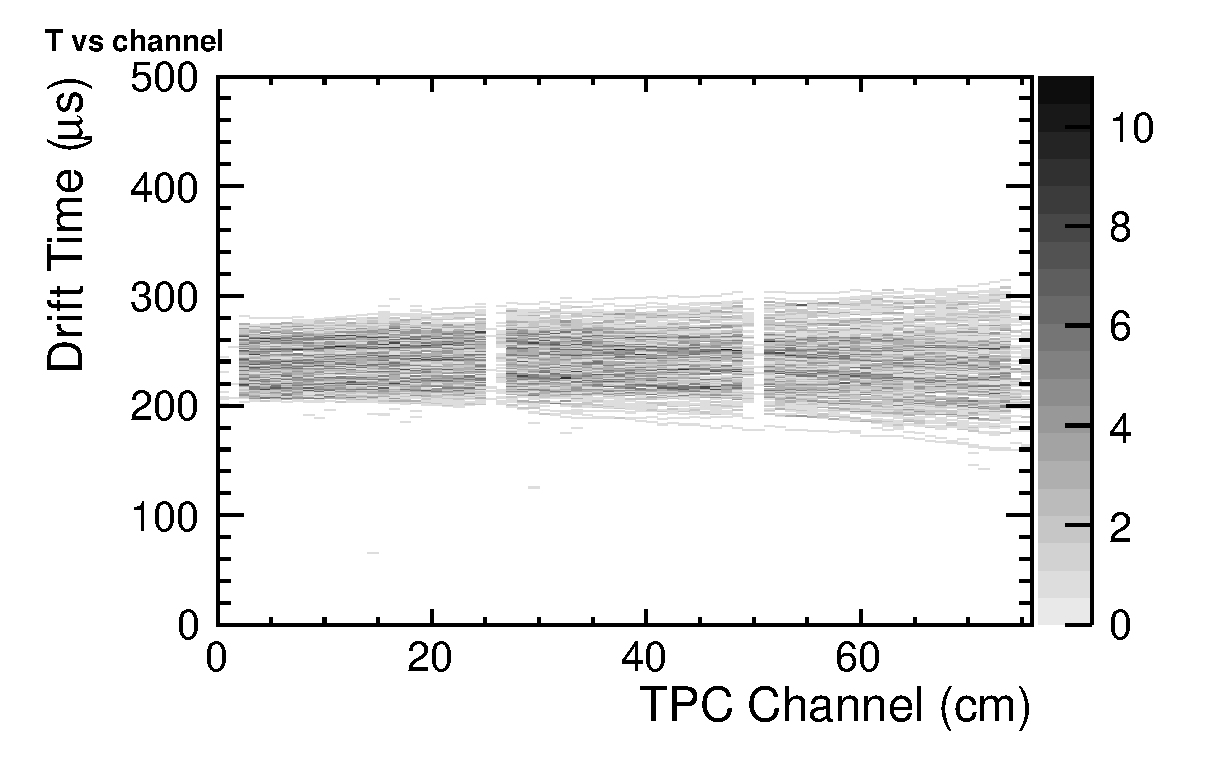
\includegraphics[width=100mm]{fig/PionTrack.eps}
 \end{center}
 \caption{800 MeV/c pion sample}
 \label{fig:PionTrack}
\end{figure}

\begin{figure}[htbp]
 \begin{center}
  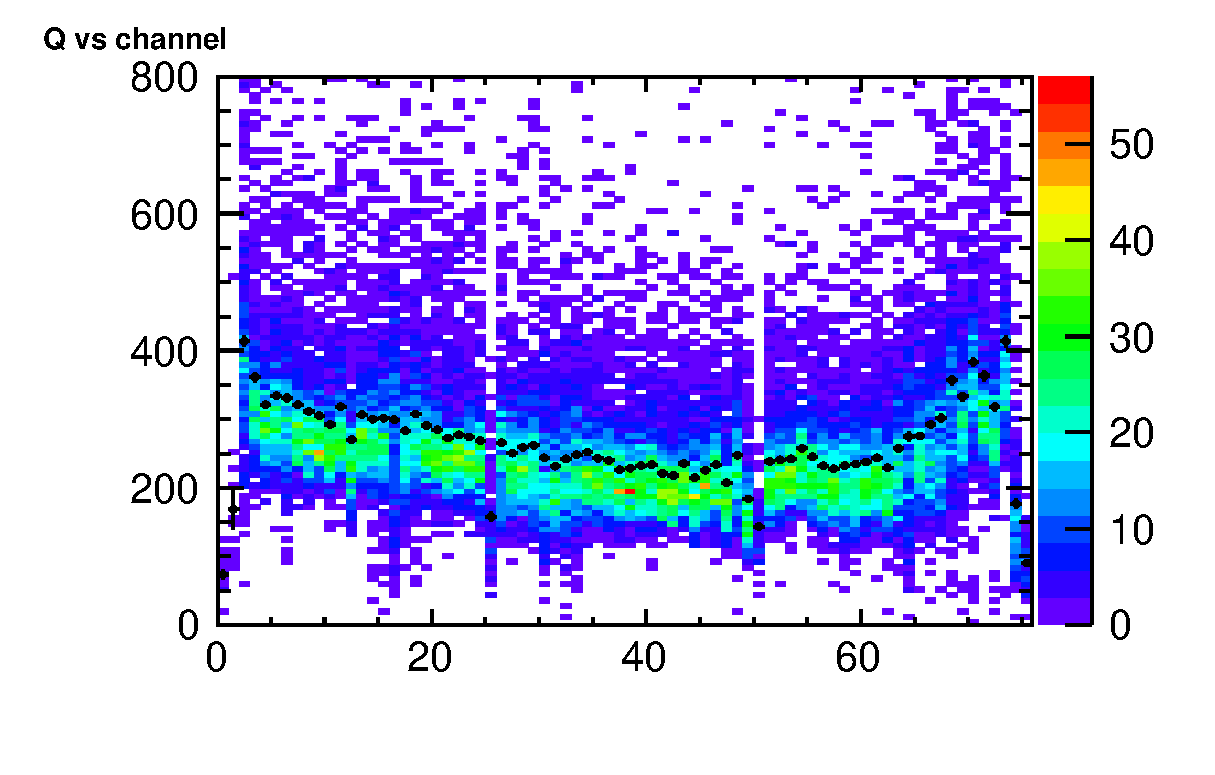
\includegraphics[width=100mm]{fig/PionQvsCh.eps}
 \end{center}
 \caption{800 MeV/c pion average hit charge}
 \label{fig:PionQvsCh}
\end{figure}

\begin{figure}[htbp]
 \begin{center}
  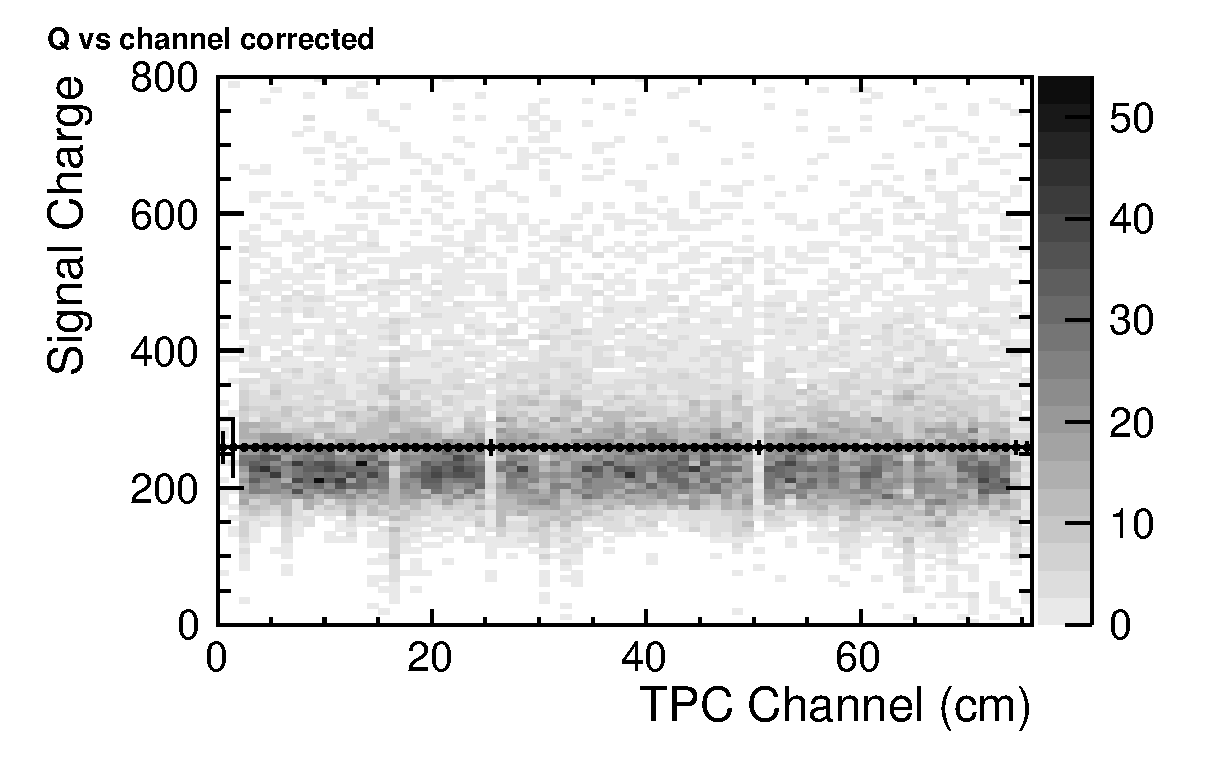
\includegraphics[width=100mm]{fig/PionQcvsCh.eps}
 \end{center}
 \caption{800 MeV/c pion average hit charge after calibration}
 \label{fig:PionQcvsCh}
\end{figure}


%%%%%%%%%%%%%%%%%%%%%%%%%%%%%%%%%%%%%%%%%%%%%%%%%%
\subsection{Liquid Argon Purity}
%%%%%%%%%%%%%%%%%%%%%%%%%%%%%%%%%%%%%%%%%%%%%%%%%%

Attenuation of the drift electron depends on purity of LAr since electronegative impurities capture it \cite{purity}. 
Thus we need to apply correction to TPC signal charge according to the drift time.
We use cosmic ray events triggered by inner PMT at off-beam timing for measuring the LAr purity, and use this to correct the beam data.
Figure~\ref{fig:CosmicEvent} shows an event display of typical cosmic muon event crossing TPC channels.
The attenuation of readout charge depending on drift time is clearly seen in the right plot. 
%Readout charge in an event cannot be fitted by exponential because energy deposition follows Landau distribution and charge readout is affected by electric field distortion which is described latter in section~\ref{sec:Efield}.
Other effects on readout charge are Landau nature in energy deposition and electric field distortion as discussed in the previous subsection.
We use multiple events to cancel Landau effect and apply channel response correction to estimate LAr purity.

%\begin{itemize}
%\item Plot: Typical Lifetime Fit  (Naganoma)
%\item Plot: Lifetime vs Time  (Naganoma)
%\end{itemize}

\begin{figure}[htbp]
 \begin{center}
  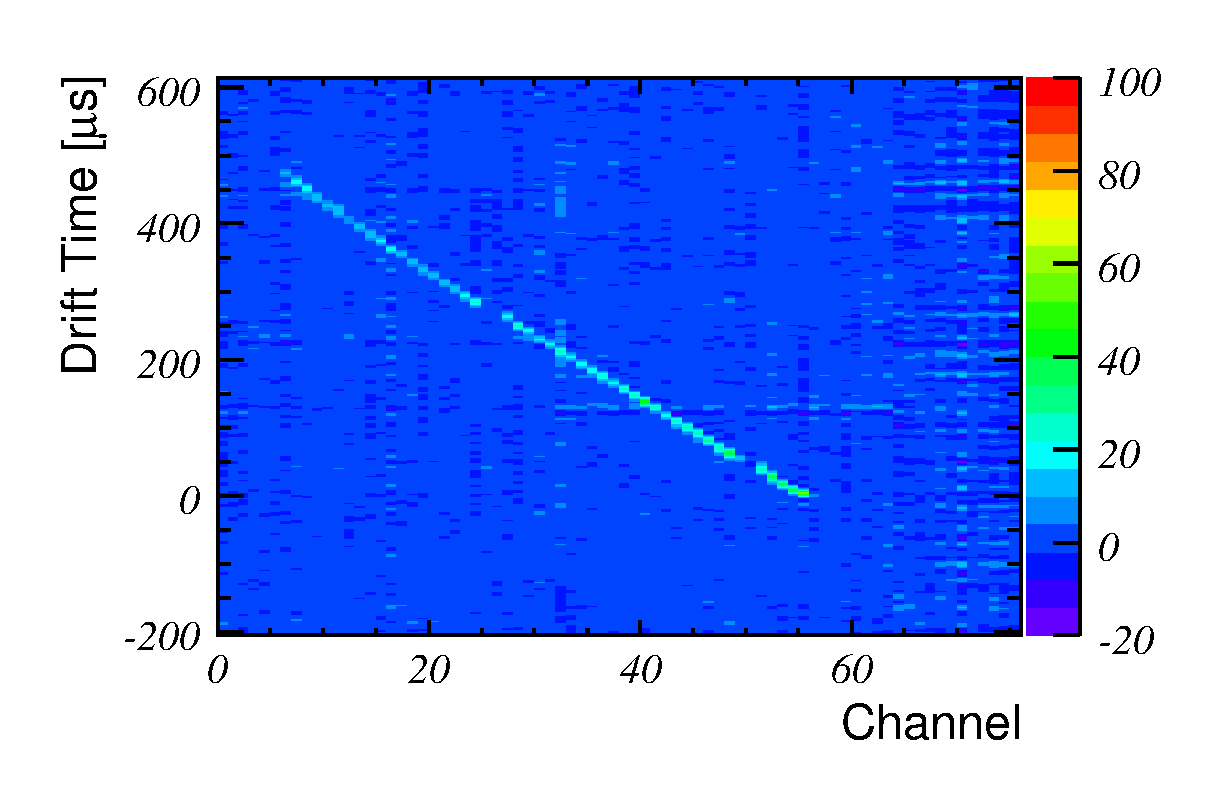
\includegraphics[width=60mm]{fig/cosmic68_ev258_display.eps}
  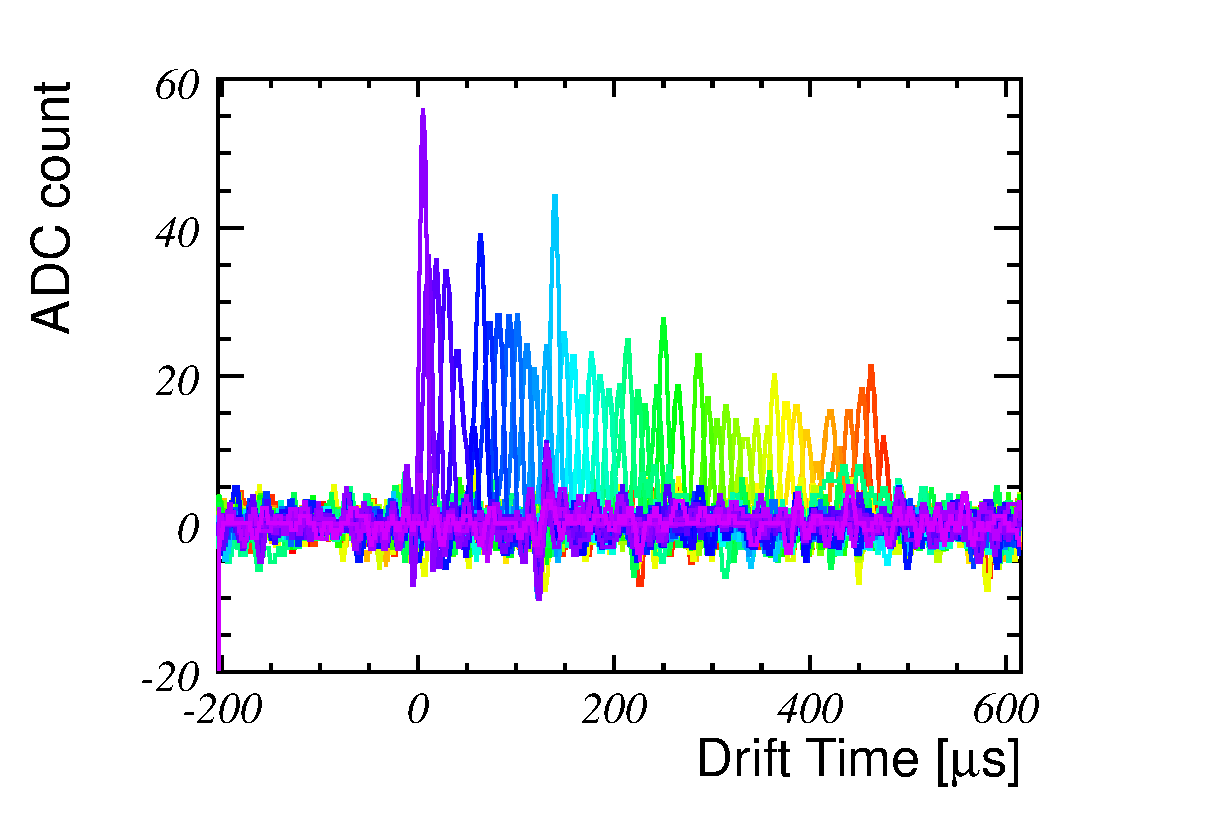
\includegraphics[width=60mm]{fig/cosmic68_ev258.eps}
 \end{center}
 \caption{Left: Typical cosmic muon event crossing TPC channels. Right: Charge deposit as a function of drift time.}
 \label{fig:CosmicEvent}
\end{figure}

We select cosmic ray event with more than 20 TPC channels which corresponds to zenith angle of more than $27^\circ$ and consistent with straight line by $\chi^2$ fit. 
Readout charge is corrected for field distortion and projected to beam direction to correct injection angle.
We fit readout charge by Landau function in each drift time bin to estimate average charge deposit. 
Figure~\ref{fig:tauExample} shows example of the average readout charge as a function of drift time which is fitted by exponential to obtain drift electron lifetime. 
%Realistic Monte Carlo simulation shows about 13\% (TBU) smaller lifetime estimation due to noise, field distortion, and FFT effects. 
%We correct output lifetime from these effects.
Figure~\ref{fig:CosmicPurity} shows an drift electron lifetime as a function of duration after initial LAr filling.
Drift electron lifetime was 600 $\mu$s at 60 hours, and 400 $\mu$s after 150 hours.
%Initial purity looks good, but the purity was slowly degrading while data taking period.
The degradation is possibly due to impurity from micro leak or out-gassing penetrating faster than purification by gas recirculation.
But we kept enough drift electron lifetime during data taking period.
The effects from noise, field distortion, and FFT give about 10\% (to be confirmed) of systematic uncertainty in LAr purity estimation.
Since charge in simulation is calibrated using through-going $\pi$ data as described later and duration of analyzed beam data is short (about 30 hours), this uncertainty gives negligible effects (to be updated, show percentage) in beam data analysis. 

\begin{figure}[htbp]
 \begin{center}
  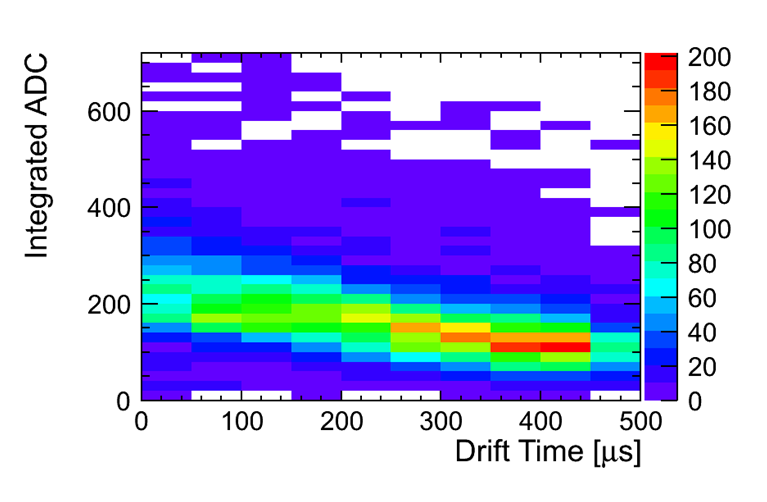
\includegraphics[width=60mm]{fig/chargeDep.eps}
  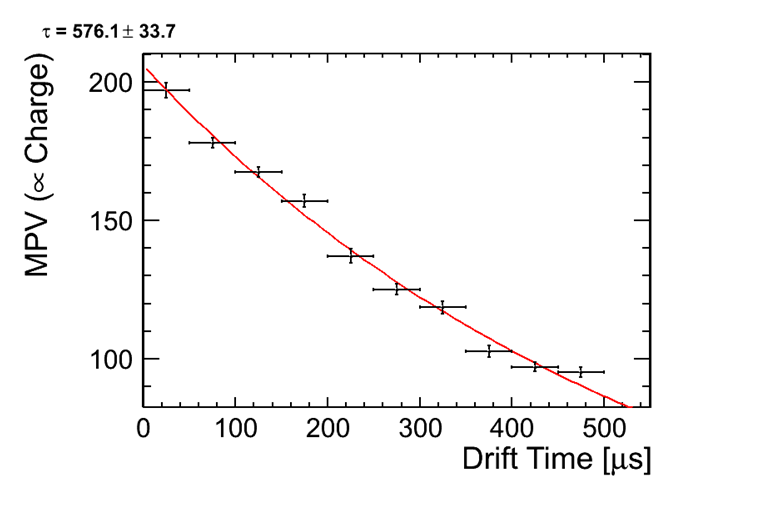
\includegraphics[width=60mm]{fig/tauExample.eps}
 \end{center}
 \caption{Left: Readout charge as a function of drift time. Readout charge in each drift time bin is fitted by landau function. Right: Average charge readout as a function of drift time which is fitted by exponential to estimate drift electron lifetime.}
 \label{fig:tauExample}
\end{figure}


\begin{figure}[htbp]
 \begin{center}
  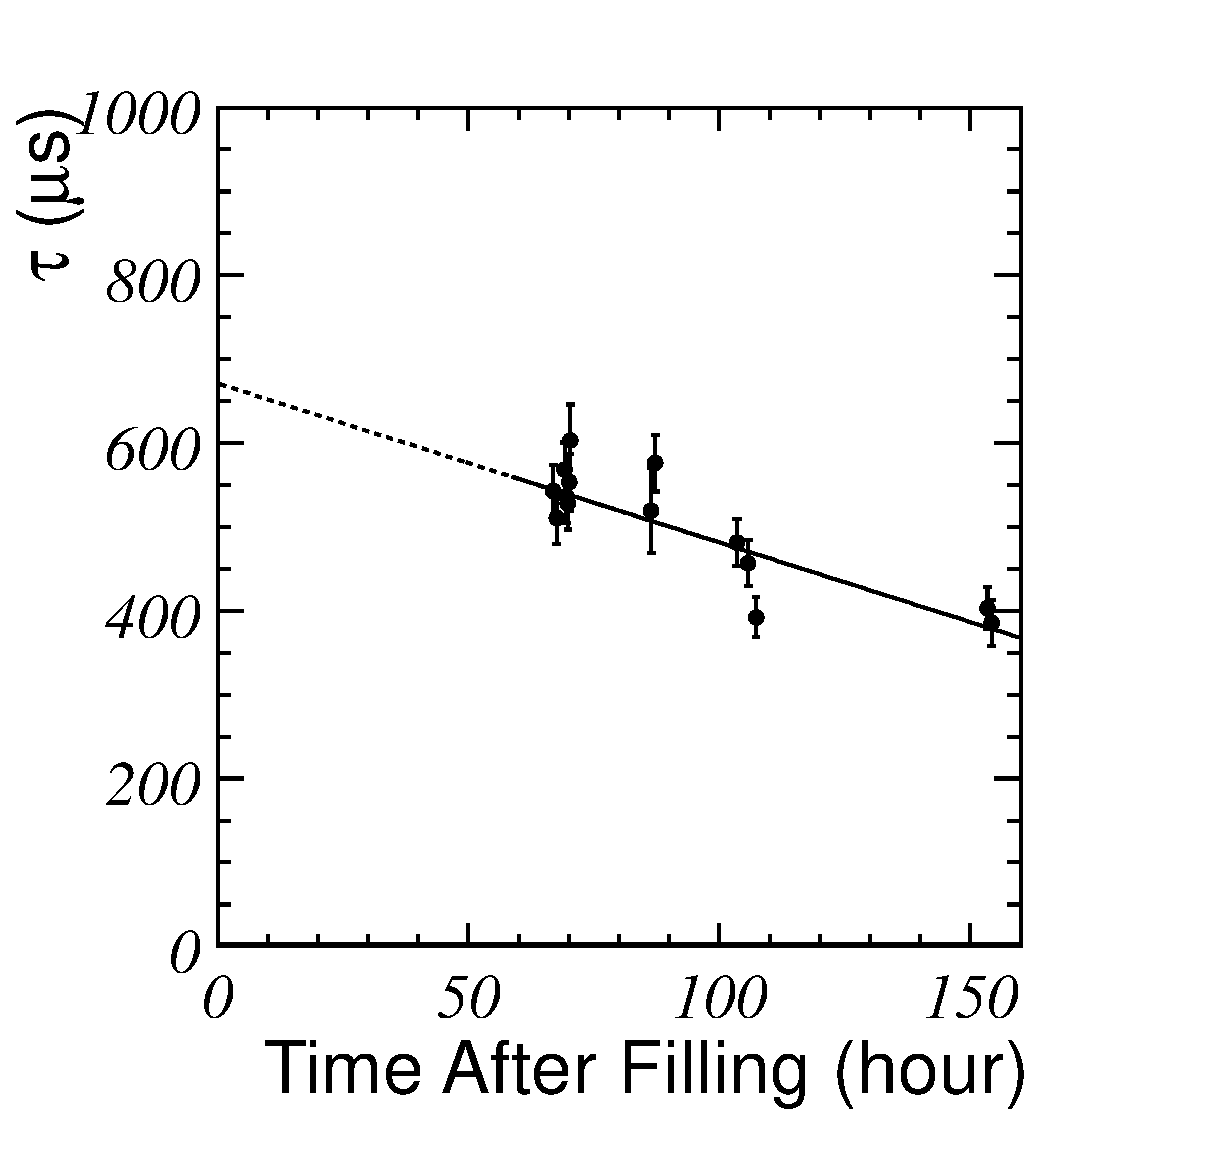
\includegraphics[width=50mm]{fig/tauHistory.eps}
 \end{center}
 \caption{Drift electron lifetime as a function of duration after initial LAr filling. The lifetime is used to correct the beam data.}
 \label{fig:CosmicPurity}
\end{figure}


%%%%%%%%%%%%%%%%%%%%%%%%%%%%%%%%%%%%%%%%%%%%%%%%%%
%\section{Event Simulation}
%%%%%%%%%%%%%%%%%%%%%%%%%%%%%%%%%%%%%%%%%%%%%%%%%%
%%%%%%%%%%%%%%%%%%%%%%%%%%%%%%%%%%%%%%%%%%%%%%%%%%
\section{Event Simulation}
%%%%%%%%%%%%%%%%%%%%%%%%%%%%%%%%%%%%%%%%%%%%%%%%%%
\subsection{Geant3, recombination, drift velocity}

We use GEANT3 for simulating energy deposition of beam particles and
their daughters. Readout pitch is 1 cm, 

we set the maximum step of Geant to 0.5 mm
which is enough smaller than the readout pitch of 1 cm.

It means charge deposition in one strip is typically 
simulated with 20 GEANT steps.

We set energy cut-off for soft electron/photon emission to
10 keV which is minimum possible energy can be set in GEANT3.
This cut-off is very important for  ionization electron recombination.

Recombination of electron and Argon ion depends on
the electric field and $dE/dx$. We use a measurement in Ref.\cite{658352}.
\begin{equation}
Q = A \frac{Q_0}{1 + k dE/dx}, A = 0.800, k = 0.486
\end{equation}

Velocity of the drift electron depends on the liquid Argon temperature
and the electric field. We use a measurement in Ref \cite{649233}.


\begin{verbatim}
 *     Special TPAR for TMED   3   Liquid_argon                                                    *
 *  CUTGAM= 10.00 keV  CUTELE= 10.00 keV  CUTNEU= 10.00 MeV  CUTHAD= 10.00 MeV  CUTMUO= 10.00 MeV  *
 *  BCUTE = 10.00 keV  BCUTM = 10.00 keV  DCUTE = 10.00 keV  DCUTM = 10.00 keV  PPCUTM= 10.00 MeV  *
 *  IPAIR=  1.  ICOMP=  1.  IPHOT=  1.  IPFIS=  0.  IDRAY=  1.  IANNI=  1.  IBREM=  1.  IHADR=  4. *
 *  IMUNU=  1.  IDCAY=  1.  ILOSS=  1.  IMULS=  1.  IRAYL=  0.  ILABS=  0.  ISYNC=  0.  ISTRA=  0. *
\end{verbatim}



\begin{itemize}
\item Plot: Geant Geometry, typical track (Tanaka)
\item Plot: recombination factor, drift velocity  (Tanaka)
\end{itemize}

\subsection{Electric Field}

Electric field of the TPC field cage
We have calculated the electric field using a 2D FEM (Finite Element Method) package \cite{Ref:FEMTET}.

This field map is used for simulating electron drift.


\begin{itemize}
\item Plot: 2D field map  (Tanaka)
\end{itemize}

\subsection{Drift Electron Diffusion}
\begin{itemize}
\item Plot: drift simulation  (Tanaka)
\end{itemize}

\subsection{Preamp Gain Calibration}
\begin{itemize}
\item Preamp gain vs channel number  (Naito)
\end{itemize}

%\subsection{FFT Noise}
\subsection{FFT Noise}
There are two kind of noise in the data we obtained, random noise and coherent noise.
Random noise is the noise which exists in each anode channel.
Coherent noise is in each board.
The pseudo noise we implemented in Monte Carlo simulation is composed of random and coherent noise by this reason.

Random noise is generated from FFT(Fast Fourier Transform) distribution of real data. Figure \ref{example10ch} shows an example of FFT distribution.

Coherent noise is generated board by board as the noise scale in the real data we obtained.
The noise scale is defined as a root mean square of pedestal, minimun noise scale is about 3 and maximum noise scale is about 10 in the data.

The ratio of random and coherent noise is 1:1 as equation \ref{PseudoNoise}.
Figure \ref{coherentNoise} shows real data noise and pseudo noise we implemeted in Monte Carlo simulation.
\begin{equation}
  Pseudo\,Noise = \frac{Random\,Noise + Coherent\,Noise}{2}
  \label{PseudoNoise}
\end{equation}

\begin{figure}[!htb]
  \centering
  \centering
  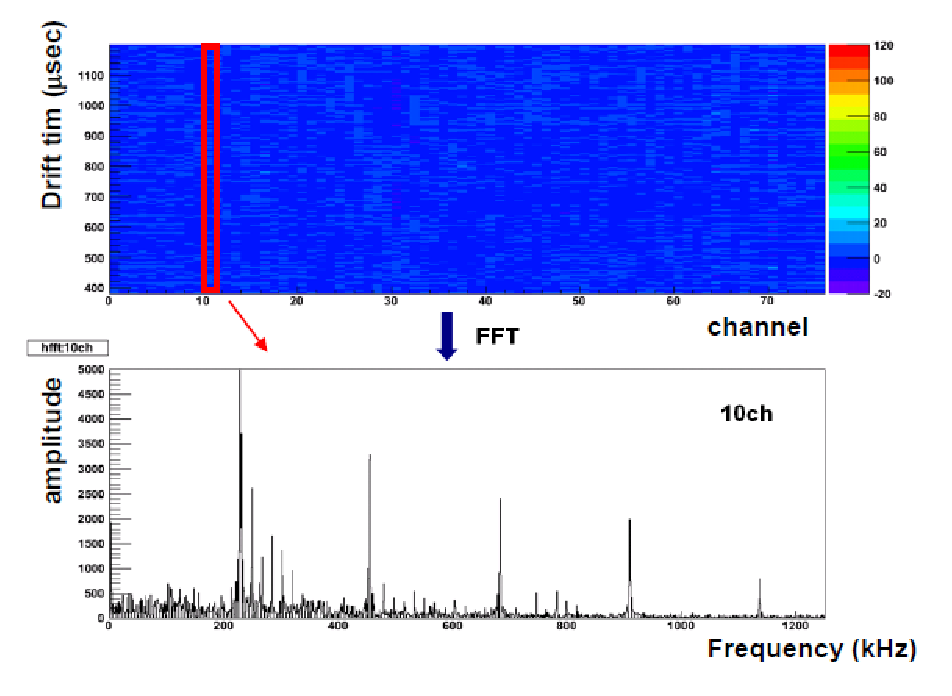
\includegraphics[width=7cm,clip]{./fig/example10ch.eps}
  \caption{example distribution of frequency:10ch}
  \label{example10ch}
\end{figure}
%\begin{figure}[!htb]
%  \centering
%  \centering
%  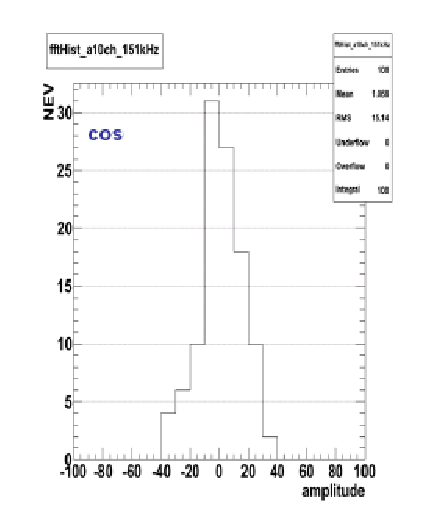
\includegraphics[width=11cm,clip]{./fig/cos.eps}
%  \caption{An example of distribution of amplitude}
%  \label{ampDist}
%\end{figure}
%\begin{figure}[!htb]
%  \centering
%  \centering
%  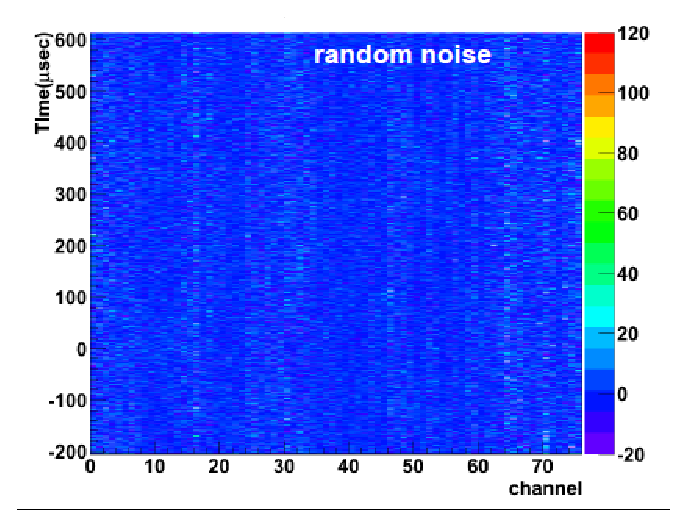
\includegraphics[width=11cm,clip]{./fig/randomnoise.eps}
%  \caption{Random noise}
%  \label{randomNoise}
%\end{figure}
\begin{figure}[!htb]
  \centering
  \centering
  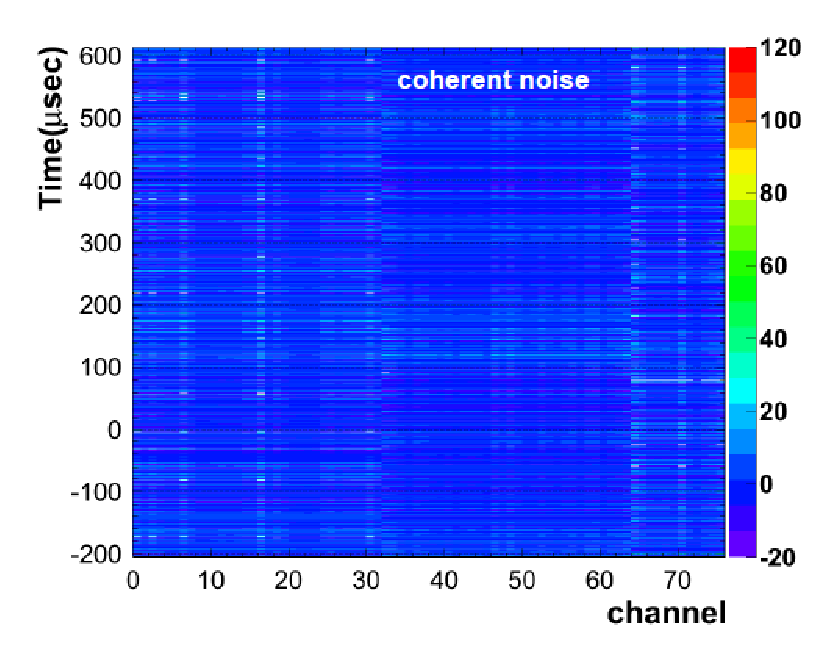
\includegraphics[width=7cm,clip]{./fig/coherentNoise.eps}
  \caption{Coherent noise}
  \label{coherentNoise}
\end{figure}
%\begin{figure}[!htb]
%  \centering
%  \centering
%  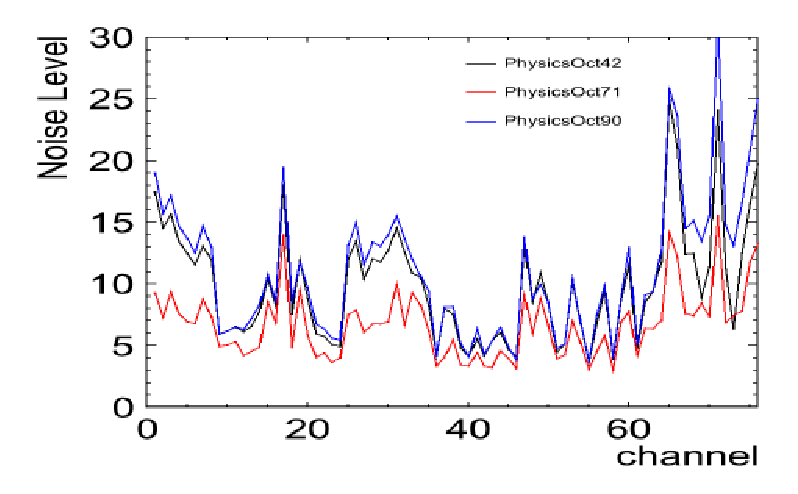
\includegraphics[width=11cm,clip]{./fig/scaling.eps}
%  \caption{Noise level}
%  \label{scaling}
%\end{figure}
\begin{itemize}
\item Plot: simulated event  (Nagasaka)
\end{itemize}

\subsection{Cross Talk}
\begin{itemize}
\item Plot: signal waveform (proton stopped point + 1)  (A. Okamoto)
\item Plot: simulated event with and without cross talk (A. Okamoto)
\end{itemize}

\subsection{Signal and Noise Scale Tuning}
\begin{itemize}
\item Plot: Landau distribution after the tuning  (Tanaka)
\end{itemize}


%%%%%%%%%%%%%%%%%%%%%%%%%%%%%%%%%%%%%%%%%%%%%%%%%%
%\section{Data-MC Comparison}
%%%%%%%%%%%%%%%%%%%%%%%%%%%%%%%%%%%%%%%%%%%%%%%%%%
%%%%%%%%%%%%%%%%%%%%%%%%%%%%%%%%%%%%%%%%%%%%%%%%%%
\section{Data- MC Comparison}
%%%%%%%%%%%%%%%%%%%%%%%%%%%%%%%%%%%%%%%%%%%%%%%%%%
\subsection{Through-going Pion}
\begin{itemize}
\item Plot: Data-MC comparison  (Tanaka)
\end{itemize}

%\subsection{Stopped Proton}
\subsection{Stopped Proton}

When we indicate the validity of charge response in high dE/dx region, proton is good sample due to its simple event structure.
At the same time, we verificate the recombination factor by proton in this analysis because proton has wide dE/dx range, and this is meaningless if the charge response of MC doesn't agree with that of DATA.
Therefore proton is very impotant in terms of comprehension of charge response.\\

First, protons are selected by the information of beam counters.
Then, proton events are applied following simple selections.\\

\begin{enumerate}
\item The drift time of the hit of the minimum channel number in the cluster is between 150$\mu$s$\sim$300$\mu$s(this time window is signal region). \\
\item The minimum channel number of hits in the cluster is below 2. \\
\item The maximum channel number of hits in the cluster is below 60. \\
\item The total hit number in the cluster is 5 or more. \\
\item The number of hits which are in the same channel is only one. \\
\end{enumerate}

We define the events which the number of clusters in the event which passed above selections is only one as good proton events.
For good proton events, we compare each paremeters of DATA and MC.
Figure\ref{fig:various_distribution} shows the comparison of the distribution of Hit Charge, Hit Sigma, Stopped Channel and  Cluster Charge between DATA and MC.
Table\ref{tb:various_distribution_comparison} shows the comparison of the mean of these distribution.

\begin{table}
  \centering
  \begin{tabular}[htb]{ccccccc}\hline
                        & DATA             & MC              & DATA/MC ratio       \\ \hline
    Hit Charge          & 607.5$\pm$19.6   & 622.3$\pm$0.8   & 0.9762$\pm$0.0316   \\
    Hit Sigma($\mu$s)   & 3.838$\pm$0.003  & 3.881$\pm$0.002 & 0.9889$\pm$0.0009   \\
    Stopped Channel     & 18.16$\pm$0.20   & 17.72$\pm$0.11  & 1.0247$\pm$0.0132   \\
    Cluster Charge      & 9940$\pm$407     & 9735$\pm$59     & 1.0210$\pm$0.0422   \\ \hline
  \end{tabular}
  \label{tb:various_distribution_comparison}
  \caption{Comparison of the mean of four distributions between DATA and MC}
\end{table}

All four distribution of MC reproduce DATA well.
Especially, the agreement of stopped channel distribution indicates the success of the momentum estimation by TOF infomation because where proton stopped depends on the initial momentum.\\

\begin{figure}[htbp]
  \centering
  \includegraphics[width=10cm,clip]{./fig/stop_proton1.eps}
  \caption{DATA-MC comparison of Hit Charge, Hit Sigma, Stopped Channel, Cluster Charge}
  \label{fig:varios_distribution}
\end{figure}

Figure\ref{fig:ADC_distribution} shows the integrated ADC distribution of each channel from stopped channel.
The MC distribution of the channels after stopped channel are good agereements with DATA.\\
The left of figure\ref{fig:Mean_comparison} shows the mean of the above distribution of each channel.
The right of figure\ref{fig:Mean_comparison} shows the ratios of DATA/MC.
The ratios are surpressed within 94\%$\sim$105\%.
From this result, we succeed in reproducing the charge response of DATA in high and wide dE/dx region.

\begin{figure}[htbp]
  \centering
  \includegraphics[width=10cm,clip]{fig/stop_proton2.eps}
  \caption{Integrared ADC distribution of each channel from stopped channel}
  \label{fig:ADC_distribution}
\end{figure}

\begin{figure}[htbp]
  \centering
  \includegraphics[width=10cm,clip]{fig/stop_proton3.eps}
  \caption{DATA-MC comparison of the mean of Integrated ADC distribution}
  \label{fig:Mean_comparison}
\end{figure}



%\subsection{Recombination Factor}
\subsection{Recombination Factor}
%In this analysis, we use parameters of the Recombination factor in a measurement of Ref.\cite{658352}.
 Electron-ion recombination depends on the electric field and stopping power $dE/dx$. We have studied this factor using tagged proton beam. Recombination factor measurement using proton beam is relatively easy because of stability of proton. This is why we used proton beam for this study as a first step.\\
  Expression for recombination can be derived 

\begin{equation}
  Q = A\frac{Q_{0}}{1+(k/E)\times(dE/dx)\times(1/\rho)}
\end{equation}

where $Q_{0}$ is initial ionization charge, E is electric field, $dE/dx$ is energy deposit per distance, $\rho$ is density of liquid Argon, A and k are fit parameters. This formula can be rearranged like below:

\begin{equation}
  \frac{Q_{0}}{Q} = \frac{1}{A}+\frac{(k/E)(dE/dx)(1/\rho)}{A}
\end{equation}

The ratio of $Q_{0}/Q$ depends on stopping power $dE/dx$, so we determined fit parameter A and k using proton data and Monte Carlo simulation. In this analysis, we need $Q$, $Q_{0}$ and $dE/dx$ channel by channel. First, Electric Field E is fixed at 0.196 [kV/cm]. Second, $Q$ is integrated charge in an anode readout channel. we can get this value from Real DATA. Third, $Q_{0}$ is integrated charge without recombination factor in an anode readout channel. This value can be obtained using Qscan. And then, $dE/dx$ per an anode channel is determined with truth information of Qscan MC. Fig\ref{fadcDist1}, \ref{fadcDistMC}, \ref{fadcDistdEdx} shows $Q$, $Q_{0}$, $dEdx$ from stopped channel -1 to stopped channel -14. In many case, integrated charge in stopped channel are composed of cross talk. This is the reason why we don't use information from stopped channel in this analysis. 

%ch by ch data distribution
\begin{figure}[!htb]
  \centering
  \centering
  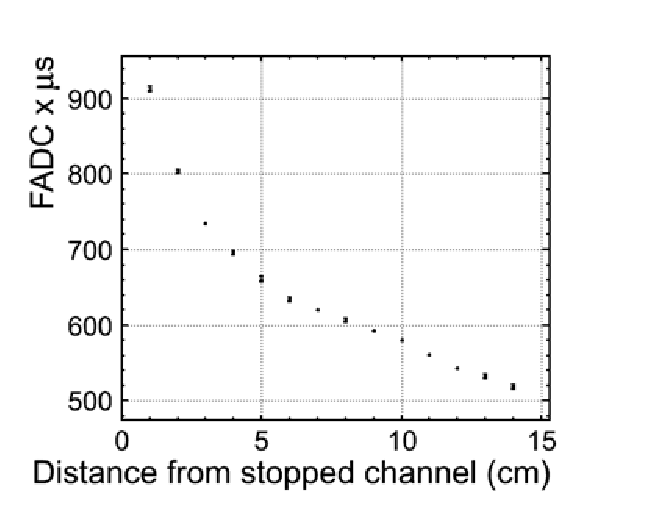
\includegraphics[width=11cm,clip]{./fig/q.eps}
%  \includegraphics[width=11cm,clip]{./fig/Data_FADCdistChbyCh.eps}
  \caption{DATA:Integrated Flash ADC counts from stopped channel -1}
  \label{fadcDist1}
\end{figure}
\pagebreak
\pagebreak

The result of this study is shown in Fig\ref{result}. Vertical axis is $Q_{0}/Q$, and horizontal axis is $dE/dx$ in this figure, this plot is fitted by Birk's low.
As a result, we got fitting parameter\\
\begin{eqnarray}
%  \center
 \nonumber  A =& 0.782\pm0.009\\
   k =& 0.0467\pm0.0009 [kV(g/cm^{2})/cm/MeV]
\end{eqnarray}

We checked Birk's low in the range 4 $[MeV/(g/cm^2)]$ $\leqq dE/dx \leqq$ 12 $[MeV/cm^2]$ and the result is consistent with ICARUS experiment's one in -- sigma.

%ch by ch MC distribution
\begin{figure}[!htb]
  \centering
  \centering
  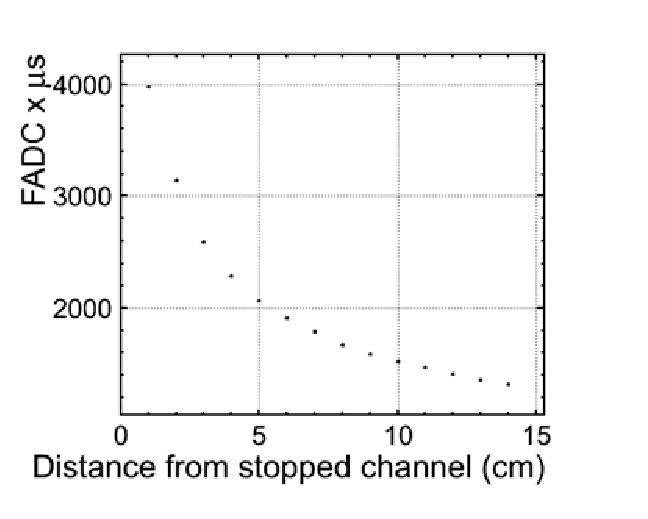
\includegraphics[width=11cm,clip]{./fig/q_0.eps}
%  \includegraphics[width=11cm,clip]{./fig/MC_FADCdistChbyCh.eps}
%  \caption{MC:Distribution of Flash ADC counts ch by ch
  \caption{MC without recombination:Integrated Flash ADC counts from stopped channel -1}
  \label{fadcDistMC}
\end{figure}

%ch by ch dE/dx distribution
\begin{figure}[!htb]
  \centering
  \centering
  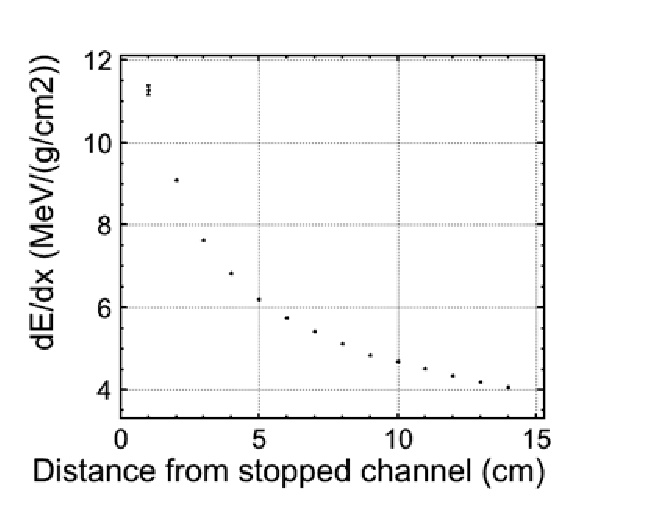
\includegraphics[width=11cm,clip]{./fig/dedx.eps}
%  \caption{Distribution of dE/dx ch by ch}
  \caption{dE/dx from stopped channel -1}
  \label{fadcDistdEdx}
\end{figure}

%result
\begin{figure}[!htb]
  \centering
  \centering
  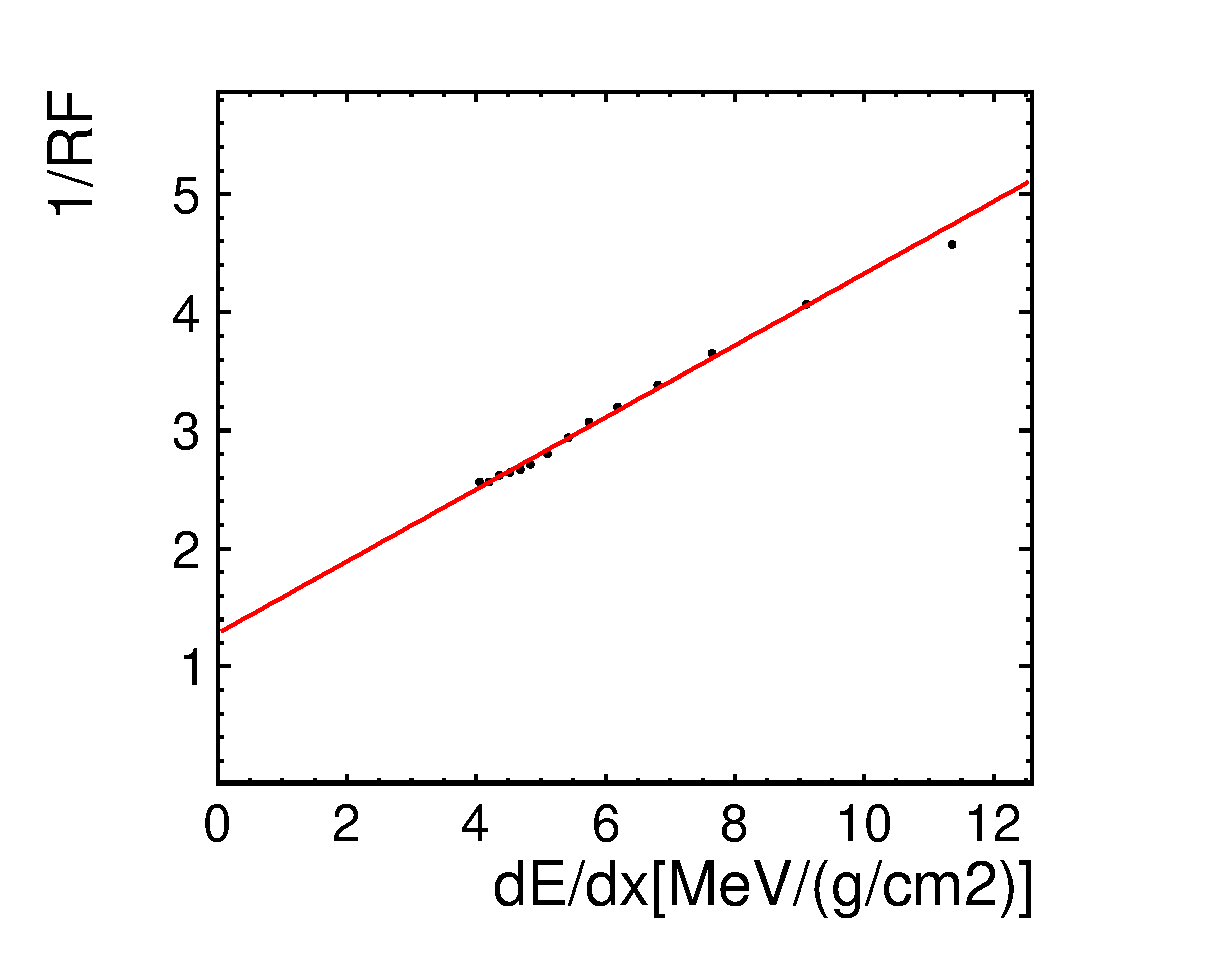
\includegraphics[width=11cm,clip]{./fig/result.eps}
  \caption{1/RF VS dE/dx: fitted by Birk's low}
  \label{result}
\end{figure}


%\subsection{Stopped Kaon}
\subsection{Stopped Kaon}
In this section , we compare some quantities of data and MC simulation that K stop in the liquid argon detector and can detect stopped point.
Figure \ref{KsomeQuantities} shows Data and MC comprison for signal hit charge , sigmal width , cluster charge and primary paricle charge distribution.
Data of signal charge and signal width are consistnt with MC one in error by less than two $\%$ and data of cluster charge and parimary charge are consistent with  MC one in error by less than five $\%$.

Figure \ref{cq27_hough} shows signal hit charge distribution of restricted channel 27. 
As it can be noiced for figure \ref{cq27_hough} , signal charge have two peaks at 300 and 500 dQ/dx.
Because two peaks has correlation of $\Delta$TOF , there is some possibility of not passig in the center of the detector.
So , we use only the event that signal charge of restricted channel 27 is less than 350.
Figure \ref{RangeVsHit_hough} shows signal hit charge distribution in different distance from the stopped point.

\begin{figure}[htbp]
  \begin{center}
    \begin{tabular}{cc}
      \resizebox{50mm}{!}{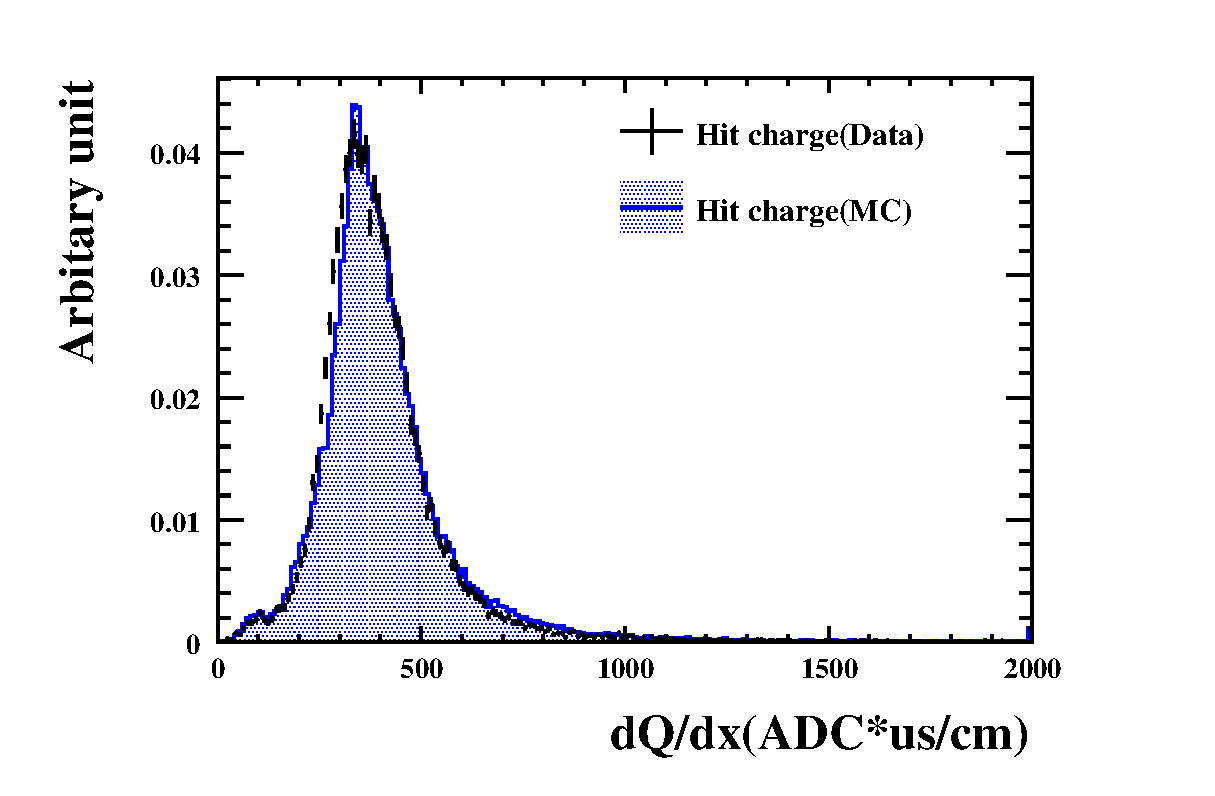
\includegraphics{fig/cHitq_hough.eps}}&
      \resizebox{50mm}{!}{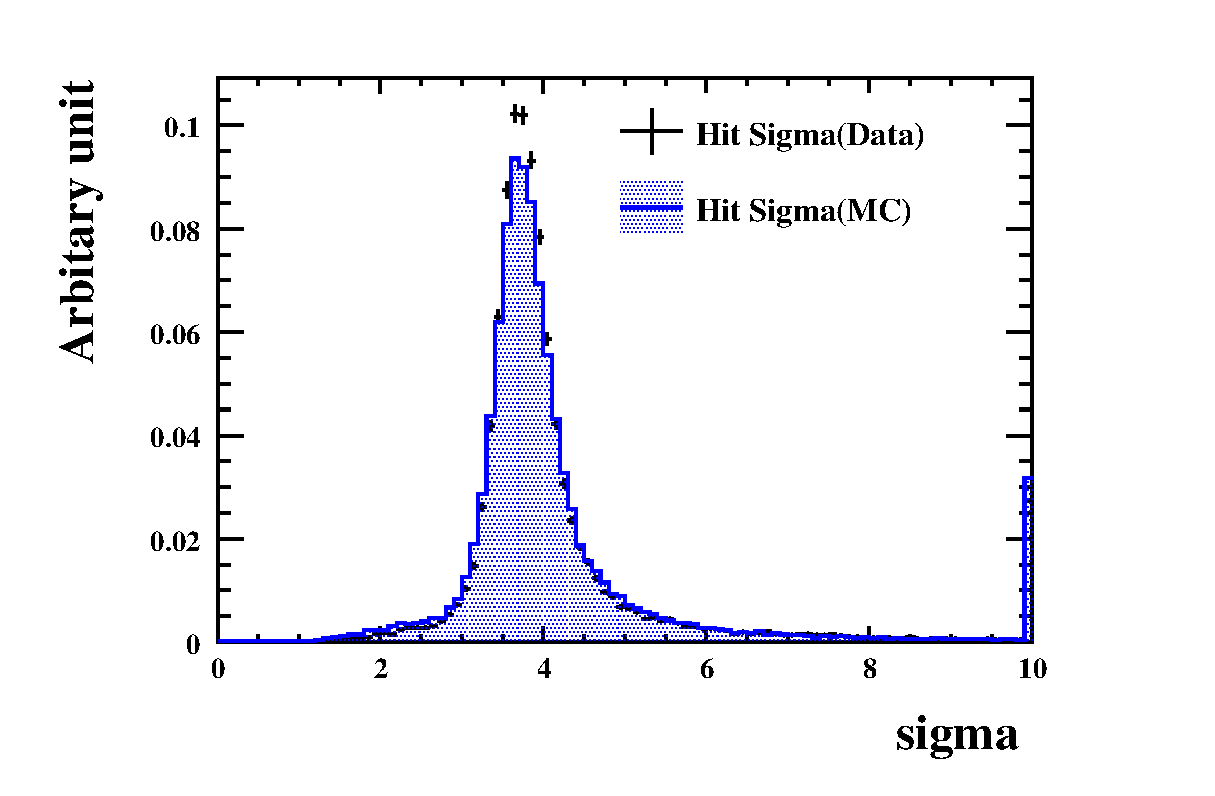
\includegraphics{fig/cHitSigma_hough.eps}}\\
      \resizebox{50mm}{!}{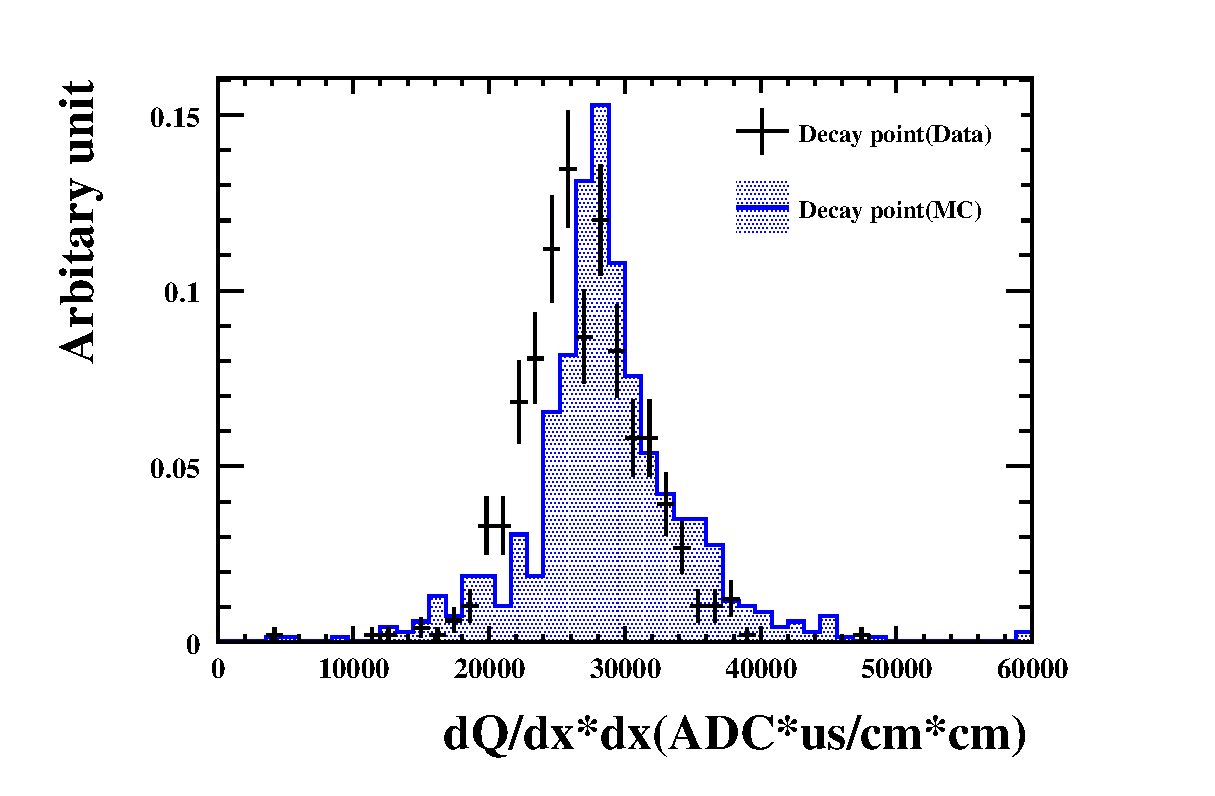
\includegraphics{fig/cClusterCharge_hough.eps}}&
      \resizebox{50mm}{!}{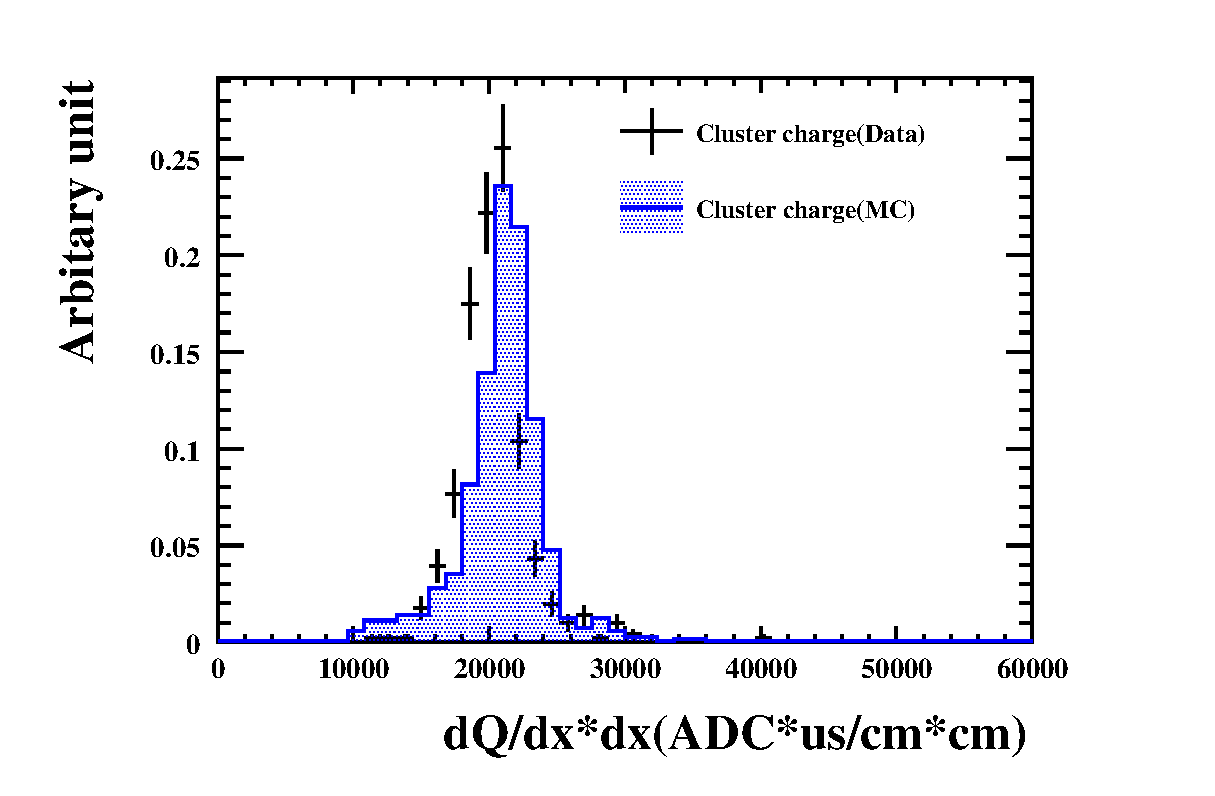
\includegraphics{fig/cCSTSP_hough.eps}}\\
    \end{tabular}
    \caption{Data-MC comparison for hit charge, hit sigma, cluster charge, primary particle charge}
    \label{KsomeQuantities}
  \end{center}    
\end{figure}
 \\


\begin{figure}[!htb]
  \begin{center}
    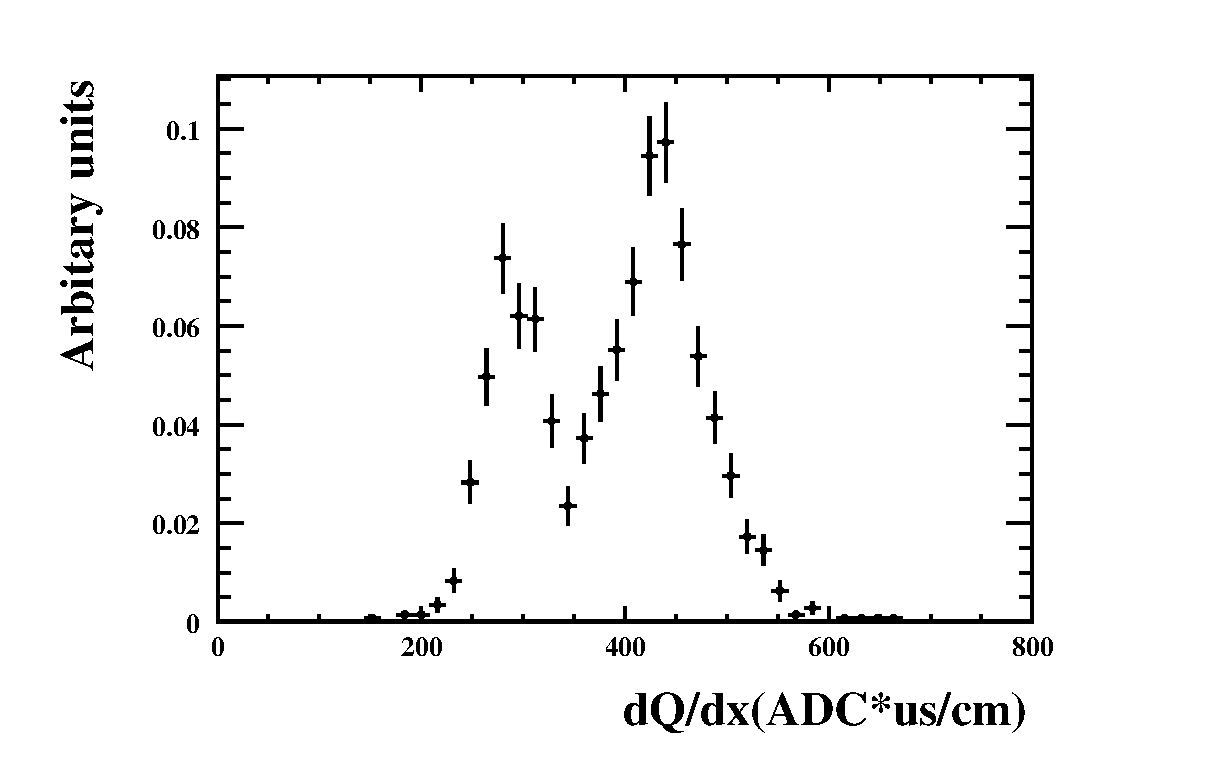
\includegraphics[width=70mm]{fig/cq27_hough.eps}
  \end{center}
  \label{cq27_hough}
  \caption{Hit charge in channel 27}
\end{figure}

\begin{figure}[!htb]
  \begin{center}
    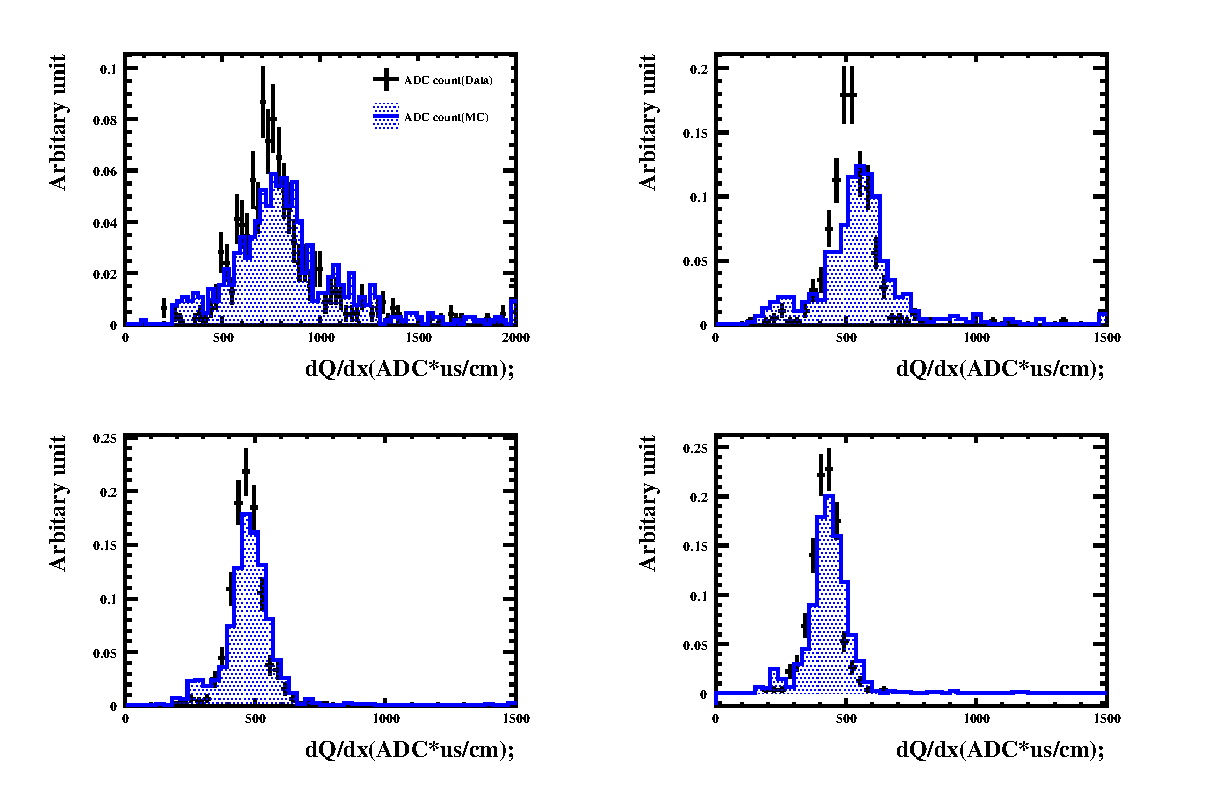
\includegraphics[width=100mm]{fig/RangeVsHit4_wcut_hough.eps}
  \end{center}
  \caption{Data-MC comparison for hit charge distribution in different distance from the stopped point(top left:decay point,top light:decay point-5cm,bottom left:decay point-10cm,decay point-15cm)}
  \label{RangeVsHit_hough}
\end{figure}

As it can be noticed for figure \ref{RangeVsHit_hough} , data plot is consistent with MC one.
Figure \ref{RangeVsHitRatio_hough} shows data/MC ratio of signal hit charge distribution in different distance from the stopped point.
Data of signal charge in dirfferent distance from stoppd point are consistnt with MC one in error by less than five $\%$ 

\begin{figure}[htb]
  \begin{center}
    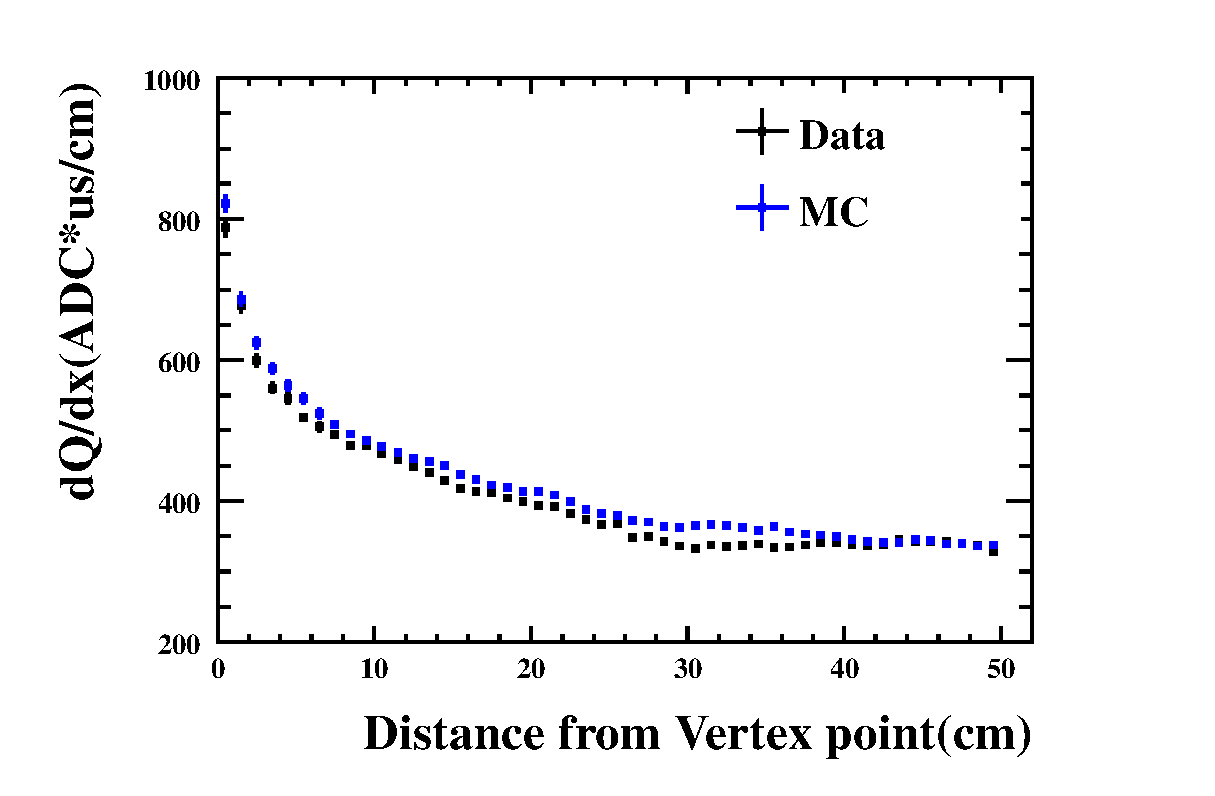
\includegraphics[width=70mm]{fig/RangeVsHitfabs_wcut_hough_ver2.eps}
  \end{center}
  \caption{Data-MC comparison for hit charge distribution in different distance from the stopped point}
  \label{RangeVsHitfabs_hough}
\end{figure}

\begin{figure}[htb]
  \begin{center}
    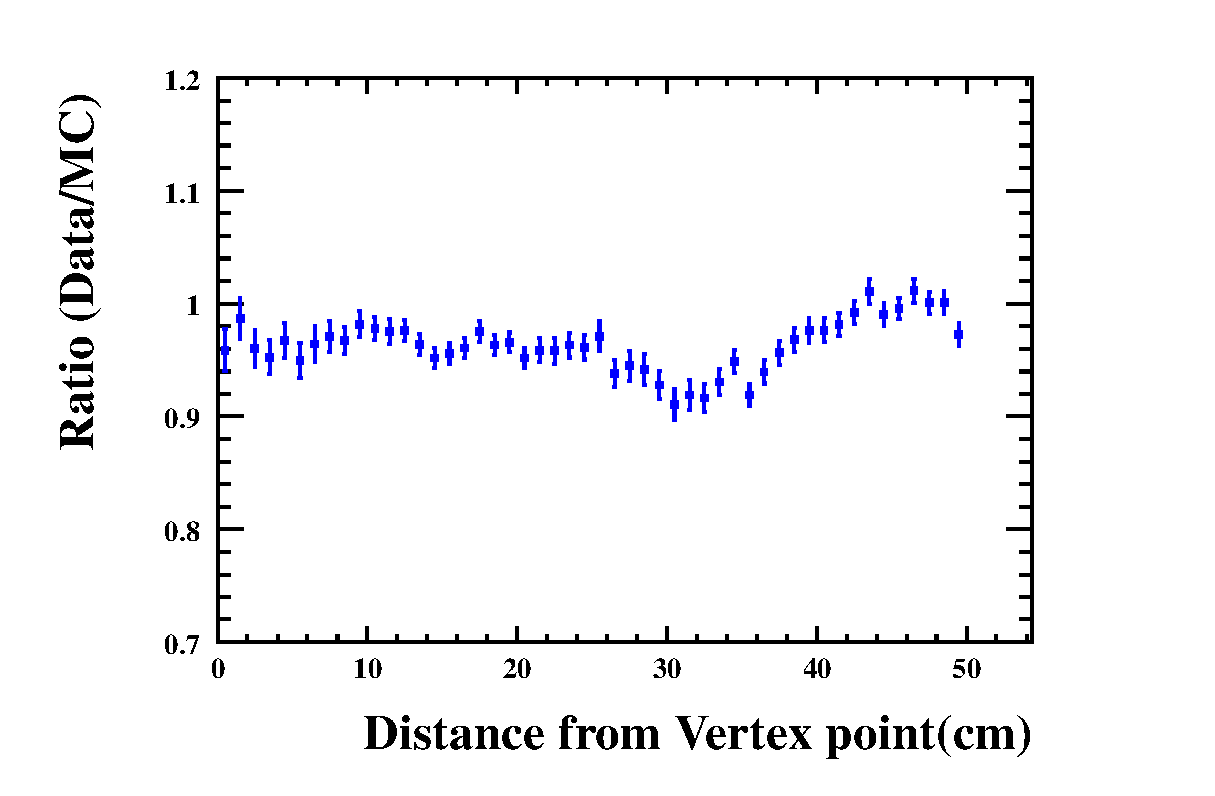
\includegraphics[width=70mm]{fig/RangeVsHitRatio_wcut_hough_ver2.eps}
  \end{center}
  \caption{Data/MC ratio for hit charge distribution in different distance from the stopped point}
  \label{RangeVsHitRatio_hough}
\end{figure}






%%%%%%%%%%%%%%%%%%%%%%%%%%%%%%%%%%%%%%%%%%%%%%%%%%
%\section{Summary}
%%%%%%%%%%%%%%%%%%%%%%%%%%%%%%%%%%%%%%%%%%%%%%%%%%
\section{Summary}
\begin{itemize}
\item We have constructed 250L LArTPC
\item Collected high purity Pion, Kaon, and proton sample
\item Establish Kaon stopped point finding algorithm
\item Develop realistic detector simulation
\item Good understanding of Pion Landau distribution
\item Good understanding of Proton and Kaon dE/dx
\item Measurement of recombination using pi, K, and proton
\end{itemize}


%% The Appendices part is started with the command \appendix;
%% appendix sections are then done as normal sections
%% \appendix

%% \section{}
%% \label{}

%% References
%%
%% Following citation commands can be used in the body text:
%% Usage of \cite is as follows:
%%   \cite{key}         ==>>  [#]
%%   \cite[chap. 2]{key} ==>> [#, chap. 2]
%%

%% References with bibTeX database:

\bibliographystyle{elsarticle-num}
\bibliography{<your-bib-database>}

%% Authors are advised to submit their bibtex database files. They are
%% requested to list a bibtex style file in the manuscript if they do
%% not want to use elsarticle-num.bst.

%% References without bibTeX database:

\begin{thebibliography}{00}

%% \bibitem must have the following form:
%%   \bibitem{key}...
%%

% \bibitem{}
%\cite{Araoka:2011pw}
\bibitem{Araoka:2011pw}
  O.~Araoka {\it et al.},
  %``A tagged low-momentum kaon test-beam exposure with a 250L LAr TPC (J-PARC
  %T32),''
  J.\ Phys.\ Conf.\ Ser.\  {\bf 308}, 012008 (2011)
  [arXiv:1105.5818 [physics.ins-det]].
  %%CITATION = 00462,308,012008;%%

\bibitem{Mihara:2004ft}
S.~Mihara [MEG Collaboration],
%``R&D work on a liquid-xenon photon detector for MEG experiment at PSI,''
Nucl.\ Instrum.\ Meth.\ A {\bf 518}, 45 (2004).
%%CITATION = NUIMA,A518,45;%%

%\cite{658352}
\bibitem{658352} 
  S.~Amoruso {\it et al.} [ICARUS Collaboration],
  %``Study of electron recombination in liquid argon with the ICARUS TPC,''
  Nucl.\ Instrum.\ Meth.\ A\ {\bf 523}, 275  (2004).
  %%CITATION = NUIMA,A523,275;%%

%\cite{649233}
\bibitem{649233} 
  S.~Amoruso, M.~Antonello, P.~Aprili, F.~Arneodo, A.~Badertscher, B.~Baibusinov, M.~Baldo-Ceolin and G.~Battistoni {\it et al.},
  %``Analysis of the liquid argon purity in the ICARUS T600 TPC,''
  Nucl.\ Instrum.\ Meth.\ A\ {\bf 516}, 68  (2004).
  %%CITATION = NUIMA,A516,68;%%

\bibitem{purity}
  A.~Bettini {\it et al.}, Nucl.\ Instrum.\ Meth.\ A\ {\bf 305}, 177 (1991).

\bibitem{3069654}
  P.V.C Hough 'Method and means for recognizing complex patterns',United States Patent Office 3069654(1962) 

\end{thebibliography}


\end{document}

%%
%% End of file `elsarticle-template-num.tex'.
